\documentclass[12pt]{iopart}
\newcommand{\gguide}{{\it Preparing graphics for IOP Publishing journals}}
\usepackage{graphicx}
%Uncomment next line if AMS fonts required
%\usepackage{iopams}  

\bibliographystyle{plain}

\begin{document}

\title[Machine Learning for Defect Identification in Crystalline Materials]{Machine Learning for Defect Identification in Crystalline Materials}

\author{Michael D Skarlinski and David J Quesnel}

\address{University of Rochester, Hopeman Engineering Building, Rochester NY, 14627}
\ead{michael.skarlinski@rochester.edu}
\vspace{10pt}
\begin{indented}
\item[]\date{\today}
\end{indented}

\begin{abstract}
Machine learning is a versatile tool for finding complex trends in large datasets. Recent developments in atomistic representations have resulted in rotationally, translationally, and permutationally invarient expressions for local atomic environments. Here we use these unique representations to collect a small database of standard crystalline defects, such as partial and full dislocations, surfaces vacancies, interstitials, and grain boundaries for both FCC and BCC materials. Both thermal perturbations and strains are included in the training data to make the final classification algorithm robust against erors in both. We develop a machine learning approach, called BiDef, to identify similar defects which were not present in the training data, which remains quite flexible for adding new defects or atomic structures. Error analysis indicates that the BiDef algorithm is more accurate than CSP and CNA methods in idenfying defects during tensile testing of nanowire samples, as well as vacancy diffusion experiments. However, the power and flexibility of the method comes at a relatively large comutational cost.
\end{abstract}

% Uncomment for PACS numbers
%\pacs{00.00, 20.00, 42.10}
%
% Uncomment for keywords
%\vspace{2pc}
%\noindent{\it Keywords}: XXXXXX, YYYYYYYY, ZZZZZZZZZ
%
% Uncomment for Submitted to journal title message
%\submitto{\JPA}
%
% Uncomment if a separate title page is required
%\maketitle
% 
% For two-column output uncomment the next line and choose [10pt] rather than [12pt] in the \documentclass declaration
%\ioptwocol
%

\section{Introduction}

\subsection{Defect Identification in Crystalline Simulations}

The fact that mechanical, electrical and optical properties of materials are largely determined by cyrstalline defects is a fundamental tenet of materials science. For example, grain boundaries can act as dislocation sources or sinks, or serve to hinder dislocation motion through a crystal, causing Hall-Petch hardening. Vancacy clusters can collapse to cause stacking faults separated by partial dislocations, and interstitial atom strain fields can inhibit dislocation motion. Energy differences among atomic planes can facilitate or retard crack formation along those particular atomistic directions. 

Molecular dynamics gives scientists an excellent tool to investigate these defect structures such as surfaces, grain boundaries, dislocations, interstitial atoms or vacancies. Since these simulations only track the trajectories of atoms, it is necessary to develop classification schemes which allow for the particular atoms contained within these defects to be identified. As simulations evolve into larger scales or complexities, the identification of defects within crystals becomes a labor intensive and sometimes imprecise task. Currently, many defect identification methods exist with a variety of applicabilities for different scenarios. Comparisions between the most popular methods are given by Stukowski\cite{Stukowski2012}.

As noted his work, geometric indicators are often used such as inter-atomic distances, bond angles or bond network topology. Popular descriptor methods include Common neighbor analysis (CNA)\cite{Honeycutt1987}, Centrosymmetry parameterization\cite{Kelchner1998}, and bond-order analysis\cite{Steinhardt1983}. We use these techniques (particularly CNA and CSP) as benchmarks for defect identification performance in this work. CNA and adaptive-common neighbor analysis \cite{Stukowski2012} are defect identification methods based on variations in the topology of bonds in the neighborhood of a given atom. The method works by taking $N$ nearest neighbors, where $N$ is 12 for FCC and HCP, 14 for BCC, and 16 for cubic diamond, and comparing three different bond properties between each of them. The three properties are, $n_{cn}$, the number of neighbor atoms shared between the central atom and each atom its bonded to, $n_b$, the number of bonds between each of these common neighbors, and $n_{lcb}$, the lowest number of bonds possible in a chain which connects the common neighbors. This set of three descriptors is used for each of the $N$ neighbors, and allows for unique identification of the local structure surrounding a particular atom. CSP\cite{Kelchner1998} analysis provides another tool for defect identification, where local bond symmetry is used as a descriptor. The centrosymmetry parameter is defined as,

\begin{eqnarray}
CSP = \sum_{i=1}^{N/2}|\mathbf{r_i}+\mathbf{r_{i+N/2}}|^2. 
\end{eqnarray}

Where $\mathbf{r_i}$ and $\mathbf{r_{i+N/2}}$ are vectors between the atom of interest and a pair of opposite neighbors. The pairs are identified by summing the bond vectors for each of the $N(N-1)/2$ possible atom pairs, and finding the $N/2$ pairs with the smallest bond magnitude, $|\mathbf{r_i} + \mathbf{r_j}|^2$. When the atom of interest is in a perfect lattice site, only symmetric pairs of opposite atoms will be chosen, giving a CSP value near zero. The less symmetric the pairs of atoms are, the higher the CSP value. Bond-order analysis \cite{Steinhardt1983} identifies defects by projecting the vectors between neighbors onto a unit sphere, then defines a set of parameters based on rotationally invariant combinations of spherical harmonics, which are charactaristic to each crystal structure. The technique was developed for identifying glass transitions in metallic glass, and it allows for charactarization between amorphous and crystalline states.

While the primary advantage of the above methods is in their speed and simplicity, they suffer from being relatively innaccurate at high temperatures or crystalline strains. Furthermore, they have little ability to uniquely identify defective structures: CNA can only determine the presence of crystal structures and CSP anlaysis will give a scalar value which is difficult to correlate to a particular defect. Some more recent methods have made strides toward unique defect identification, including the dislocation extraction algorithm (DXA)\cite{Stukowski2010b} and Topological fingerprint based analysis\cite{Schablitzki2013}. DXA allows dislocations to be completely identified within a crystalline structure. The algorithm is essentially split into three steps, fistly, ordered atoms are identified by CNA, then the defect atoms are taken and tranformed into an \emph{interface mesh}, where the perfect crystal is separated from the disordered portions. Finally, complete Burgers circuits are generated on the 2-d manifold where dislocations can then be tranformed into one dimentional lines. The method is quite robust at identifying dislocations, and even pointing out areas where non-dislocation or unidentified defects are located in the crystal. However, the method lacks the ability to classify any type of defect, and will suffer performance degredation if the CNA analysis performed is flawed at high strain values. DESCRIBE THE TECHNIQUE HERE.

While the previously mentioned techniques hace been empirically successful at identifying structural defects, we find that improvements can be made in the unique identification of defect structures. A method capable of identifying individual defects would bypass costly manual investigations into the atomic structure using visualization or post-processing techniques. For particularly large structures of 10's of millions of atoms or more, it may not even be possible for a scientist to verify defect orientations within the crystal. The frequent use of post-processing techniques (such as slip-vector analysis \cite{Zimmerman2001}) is a time consuming process for complex configurations and structures. The ability to uniquely identify different atomic configurations would allow for the dynamic assignment of regions in which the chosen inter-atomic potentials are non-tranferrable. Potentials which were parametrized for a particular defect could be focused on atoms within that defect region. This concept could be expanded by the introduction of ab-inito methods for atoms in 'un-fitted' configurations. Here we present a technique based on the use of machine learning for the specific identification of crystal defects. We demonstrate low temperature and strain sensitivity in the atomistic identification, even when simulating non-trained data. 

\subsection{Machine Learning}

Machine learning can be broadly defined as a set of algorithms that learns and make predictions based on a set of data. The algorithms build models using input data, and make predictions based on these models as opposed to following a set of pre-made instrutions.\cite{Mohri2012} The algorithms are typically separated into two catagories: supervised learning and un-supervised learning. Supervised learning works with a vectorized set of input variables, which are known as \textit{features}, that have been pre-matched to particular values or \textit{classes}. An example could be using height as a feature which represent people's ages, these data may appear as follows: $((2.5 ft | 2 yrs), ( 3 ft | 4 yrs), (3.5 ft | 6.5 yrs), ...)$. Supervised learning algorithms take these data, referred to as a \textit{training set}, and provide a model which either classifies or predicts a new value for a previously unseen feature. In the example, new, unseen, heights could be provided, and the algorithm would attempt to identify a person's age. Un-supervised learning algorithms primarily finds relationships between data without having previously specified classes. Techniques from both catagories of algorithms were used in our analysis, but this thesis primarily used supervised learning algorithms. 

The features which represent the local atomic environments are critical for this method, and each of the previously presented defect identification methods essentially creates its own feature space for defective atoms. We were seeking a complete representation of an atom's local environment such that each defect would be able to be uniquely identified. The bond-order spectrum is a nearly complete representation of an atoms local environment, however, these components only provide the spherical symmetry around each atom, the radial information is not included. There exists a more thorough approach, developed by Albert Bartók-Pártay \cite{Bartok-Partay}, where a rotationally, translationally and permutationally invarient representation is developed, which uses an expansion in bi-spectrum coefficients to represent atomic environments. These coefficients were previously used to make a dynamically quantum-accurate classical model, known as Gaussian Applied Potentials (GAP) \cite{Bartok2010a}. However, we use these same coefficients as features in a defect identification learning algorithm, rather than a force and energy determination algorithm as in GAP.

The features for this space are simply the list of bi-spectrum components for each atom in the system, and our classes are descriptions of the local atomic sites. The classes may be defect-free sites, such as bulk FCC or bulk BCC, as well as particular defects, including grain boundaries, partial dislocations, interstitial sites, or vacancies. To get a proper sampling of features for each defect of interest, we generated a large amount of training data (described in Section \label{sec:training}), ranging from 8 to 55 features per atom for several million bulk and defective sites.

A classification algorithm must be then chosen after constructing a database of features and classes. Many different supervised classification algorithms exist such as support vector classification \cite{Smola2004}, nearest-neighbor approaches \cite{Bentley1975, Omohundro1989}, naive-bayes \cite{Zhang2004}, and ensemble based methods such as random forests \cite{Breiman2001} or Ada-boost\cite{Zhu2009}. Each method differs in efficiency and applicability for a particular set of data, where consideration of data-set size, variability, and number of classifications needs to be taken into account. in considering the large size of our training set, we chose to use a nearest-neighbor KD-Tree approach \cite{Bentley1975}, as it scales well to many features. Random forest ensemble methods\cite{Breiman2001} are also evaluated in this work, despite the slow run-time these algorithms train quickly, and are able to dynamically differentiate the importance of each featured variable. Furthermore, random forest algorithms are capable of more accurate classifications than nearest-neighbor approaches, given that enough decision trees are used. Support vector machines were not invesitaged due to the increased training time required for such large data sets. A succinct summary of these classification algorithms are included in the Methods section.

An interesting advantage of this learning method is that it is fundamentally capable of identifying any reproducable atomic defect--no matter how obscure. It is capable of identifying any class for which it has trained with similar features. This means that including the effects of thermal perturbations or strains is as simple as generating the strained or thermalized structures themselves, and then adding them to the current training set. In the current prototype version of the method, it is capable of handeling thermal and strain-based fluctions, as well as the identification of a few choice defects in FCC and BCC crystals. The method's performance and variability was evaluated in identifying a list of common defects in FCC and BCC systems, when tested in applications outside the training set.

\section{Methods}
\subsection{Unique atomic representations: Bispectrum Coefficients}

Here, the method for generating a vector which uniquely identifies the local environment of an atom which is rotationally, translationally, and permutationally invarient is briefly described. It was first developed by Bartók-Pártay \cite{Bartok-Partay}, for use in a genearlized atomic potential generation scheme, known as Gaussian Applied Potentials \cite{Bartok2010a}. They have since been adapted for use in another automated interatomic potential algorithm, Spectral Analysis Method for Automated Generation of Quantum-Accurate Interatomic Potentials or SNAP. \cite{Thompson2014} The coefficients are useful in the context of machine learning, where they can be used as an efficient feature set. Without bispectrum components, or another similar invariant representation \cite{COORDINATION VECTORS}, atomic environments can only be completely described as listings of each of their spatial coordinates. This representation would give far too many features to effecitvely train a classification algorithm on a dataset. Furthermore, the lack of invariance in an euclidean coordinate representation means that many identical structures would produce totally different feature representations. These bispectrum coefficients are later used to train an algorithm based on a database of structural defects.

Firstly an atomic density function, $\rho_i(\mathbf{r})$ is established as a sum of $\delta$ functions in space:

\begin{eqnarray}
\rho_i(\mathbf{r}) = \delta(\mathbf{r}) + \sum_{r_{ii'} < R_{cut}} f_c(r_{ii'})w_{i'}\delta(\mathbf{r}-\mathbf{r_{ii'}}),
\end{eqnarray}

here $\mathbf{r_{ii'}}$ is the vector between the atom of interest, $i$ to a neighboring atom, $i'$. The coefficients $w_i$ are weighting factors to differentiate between atom types in multi-type systems. The sum occurs for all atoms within a cutoff $R_{cut}$, and $f_c(r_{ii'})$ is a smoothing function to avoid a discontinuity at $R_{cut}$. In a similar fashion to the bond-order analysis \cite{Steinhardt1983}, the angular portion of the density function can be expanded in a basis of spherical harmonic functions, $Y_m^l(\theta,\phi)$, for $l = 0, 1, 2, ...$ and $m =-l , -l +1, ..., l-1, l$. \cite{varshalovich1988} Rather than expanding the radial component in a separate set of basis functions, Bartok et al. \cite{Bartok2010a} had the insight to map the radial distance, $r$ to a polar angle $\theta_0$ defined as follows,

\begin{eqnarray}
\theta_0 = \theta_0^{max} \frac{r}{R_{cut}}
\end{eqnarray}

$\theta_0$ maps the points, $(\theta,\phi,r)$ to a a set of points on a 3-sphere (sphere analog in 4-D), $(\theta,\phi,\thea_0)$. Some $\theta_0^{max}$ value is defined to limit points to be north of this latitutde. The advantage of this trick is that 4D spherical harmonics functions,$U_{m,m'}^j(\theta_0,\theta,\phi)$, can be used as a basis set, where $j=0,\frac{1}{2},1,...$ and $m,m' = -j, -j+1, ..., j-1, j$. If the 4D harmonics functions are paramertized with Euler angles, then they become identical to Wigner D-functions from Quantum Angular Momentum. The atomic-neighbor density function can now be represented as follows,
\begin{eqnarray}
\rho(\mathbf{r}) = \sum_{j=0,\frac{1}{2},...}^{\inf} \sum_{m=-j}^j \sum_{m'=-j}^j u^j_{m,m'} U^j_{m,m'} (\theta_0,\theta,\phi)
\end{eqnarray}
The expansion coefficients can be represented as a sum since the density is comprised of delta functions,
\begin{eqnarray}
u^j_{m,m'}= U^j_{m,m'}(0,0,0) + \sum_{r_{i,i'}<R_{cut}} f_c (r_{i,i'})w_{i'}U^j_{m,m'}(\theta_0,\theta,\phi)
\end{eqnarray}
The expansion coefficients are not invariant under rotation, so a further step is taken to construct the Bispectrum coefficients,
\begin{eqnarray}
B_{j_1,j_2,j_3} = \sum_{m_1,m'_1=-j_1}^{j_1} \sum_{m_2,m'_2=-j_2}^{j_2} \sum_{m,m'=-j}^{j} (u_{m,m'}^{j}) H_{jmm', j_1m_1m'_1, j_2m_2m'_2} u^{j_1}_{m_1,m'_1} u^{j_2}_{m_2,m'_2}
\label{eqn:bispec}
\end{eqnarray}
These coefficients charactarize the density correlation for points on the 3-sphere. They can be calculated by INSET WAY HERE. Here the dynamic library provided in Lammps \cite{lammps} was used for our bispectrum component calculations.

\subsection{Nearest Neighbor Classification Algorithms}

p471 in esl II

Our intention was to cluster and identify pre-labeled defect structures using bispectrum coefficients as features. Since the training set was large (about 5 million atoms), a nearest neighbor approach, which is one of the simplest classification methods, was evaluated for use in our learning algorithm. The conceptual basis behind nearest neighbor classification algorithms is quite simple, first a distance metric is defined in feature space (typically a euclidean distance). When new points are introduced to be classified, the algorithm calculates the distance metric between trained points in feature space, and choses the classification for which the majority of training points have the minimum distance. If there is a tie in the classifications of nearest-neighbors, then it is randomly chosen. An advantage of these methods is that they are purely memory based, so they do not require that any model be fit to the data.

A useful way to interpret the feasibility of a learning model for a particular dataset is to examine the relationship between variance and bias as the model parameters are adjusted. We used this analysis to optimize our model parameters. The trade-off between variance and bias in the nearest-neighbor algorithm is dictated by the choice of the number, $k$ of nearest neighbors. Having few neighbors (as few as 1, for instance) produces a model with extremely high variance, and low bias. It does not generalized well to unseen data.  By increasing the number of nearest neighbors the variance decreases, as the bias increases. Here, we varied the number of nearest neighbors considered as a classification parameter, the results of which are presented in the next section.

The process of chosing nearest neighbors can present a computaional burdon, where a brute force approach would result in calculating the distance between all $N$ training points to find the $k$ closest neighbors. This results in a total search process which operates at $O(ND)$, where $D$ is the number of features in the training set.  There are several algorithms for reducing the computational load such as the KDTree \cite{Bentley1975} and BallTree \cite{Omohundro1989}, which are $O(D*log(N))$ algorithms under the correct circumstances. These algorithms work by separating the feature space into discrete regions such that data occupying different regions will need not be considered as a nearest neighbors. The algorithm used here was the BallTree \cite{Bentley1975} for $D>20$ and the KDTree for smaller dimension (lower $2j$ values).

\subsection{Random Forests Classification Ensembles}

Algorithms305 in ESLII!!

Random Forests \cite{breiman2001_in_book} are an ensemble method, which implies that the classification desicion is made on the basis of an ensemble of slightly-varying simpler methods. For the aptly-named random forest, the classification is based on an ensemble of descision tree classifiers. \cite{eslii chapter} A desicion tree is a structure which divides up a feature space into rectangular regions on the basis of minimizing the node-impurity of the tree. The tree is constructed by recursively splitting the data into two parts, where each portion minimizes some function in analagy to the loss function for regression problems. The splits are made on one dimension in feature space. Ultimately the tree is left with nodes from each split decision, which lead down to terminal or leaf nodes, where the splitting stops. Chosing when to stop the tree growth can control the variance and bias of the model. Here, we stop growth when the splitting decision would produce a leaf node with fewer members than some minimum value. By adjusting this value, we can control for overfitting and bias within our model. 

The node impurity being minimized is known as a Gini index. Given some set of classifications with values $k=1,2, ..., K$, and a particular tree node $m$, the Gini index is defined as follows:

\begin{eqnarray}
Gini=\sum_{k \neq k'} \hat{p}_{mk}\hat{p}_{mk'} = \sum_{k=1}^{K} \hat{p}_{mk}}(1-\hat{p}_mk) \\
\hat{p}_mk =\frac{1}{N_m} \sum{x_i \in R_m} I(y_i = k)
\end{eqnarray}

Where $\hat{p}_{mk}$ is the proportion of each class, $k$, that is present in node $m$. The classifier works by assigning the majority class, $k(m) = arg max_k \hat{p}_{mk}$, to each member of node $m$. The Gini index is sensitive to non-majority class probabilities, such that node splits which minimize the probability of the non-majority nodes will best minimize the index. The algorithm iterates through node choices in feature space (across the range of points in each feature dimension), and choses a split which minimizes the Gini index. This continues until the stop criteron is met.

The final created tree is useful because it naturally splits the data into probabilistic catagories, and it inherently finds feature importances. It is able to find feature importances because features which produce a lot of variance, or correlate well, with the classification data, will be chosen as splitting nodes much more frequently. Since the trees will continue to find nodes until some stopping criteron is reached, they are quite prone to overfitting. They are also prone to instability, as small variations in data structure can cause entirely different node choices and trees to form.

Random Forests are a system where the disadvantages of the descision trees can be minimized by combining a large number of 'de-correlated' trees, and averaging the results. The de-correlation is enforced by choosing a limited subset of features for the construction of each tree. We used a typical choice in the Random Forest, where $\sqrt{n}$ features were used for each tree, where $n$ is the total number of features. Classifications are chosen by running the entire ensemble of trees (here we used 1000) and chosing the class which was chosen by the majority.

\subsection{Training Set Construction}
\label{sec:training}

The learning algorithms required ample training data where crystalline defects were correctly identified such that they could be the proper features could be labelled. The following crystal defects were created to train the algorithm: vacancies, interstitialcies, surfaces ((111), (112), (110), (100)), partial dislocations, full dislocations, and randomly oriented grain boundaries. Each of the defects were generated for both FCC and BCC systems. The effects of temperature were included by adding random displacements between 0 and 0.04 $\AA$ on each atom, and generating 20 copies of each defect with different random configurations. Normal strains were also included by straining the cell in all combinations of $\hat{x}$, $\hat{y}$, and $\hat{z}$ directions at both 5\% and 10\% strains. Dislocations were created by applying burgers vectors within material slabs using the atomsk \cite{Hirel2015} code. The partial dislocations were of the $b=\frac{a_0}{6}<112>$ type for FCC. The full dislocations were of $b=\frac{a_0}{2}<110>$ and $b=\frac{a_0}{2}<111>$ for FCC and BCC cells, respectively.

\begin{figure}[htbp]
  \centering
    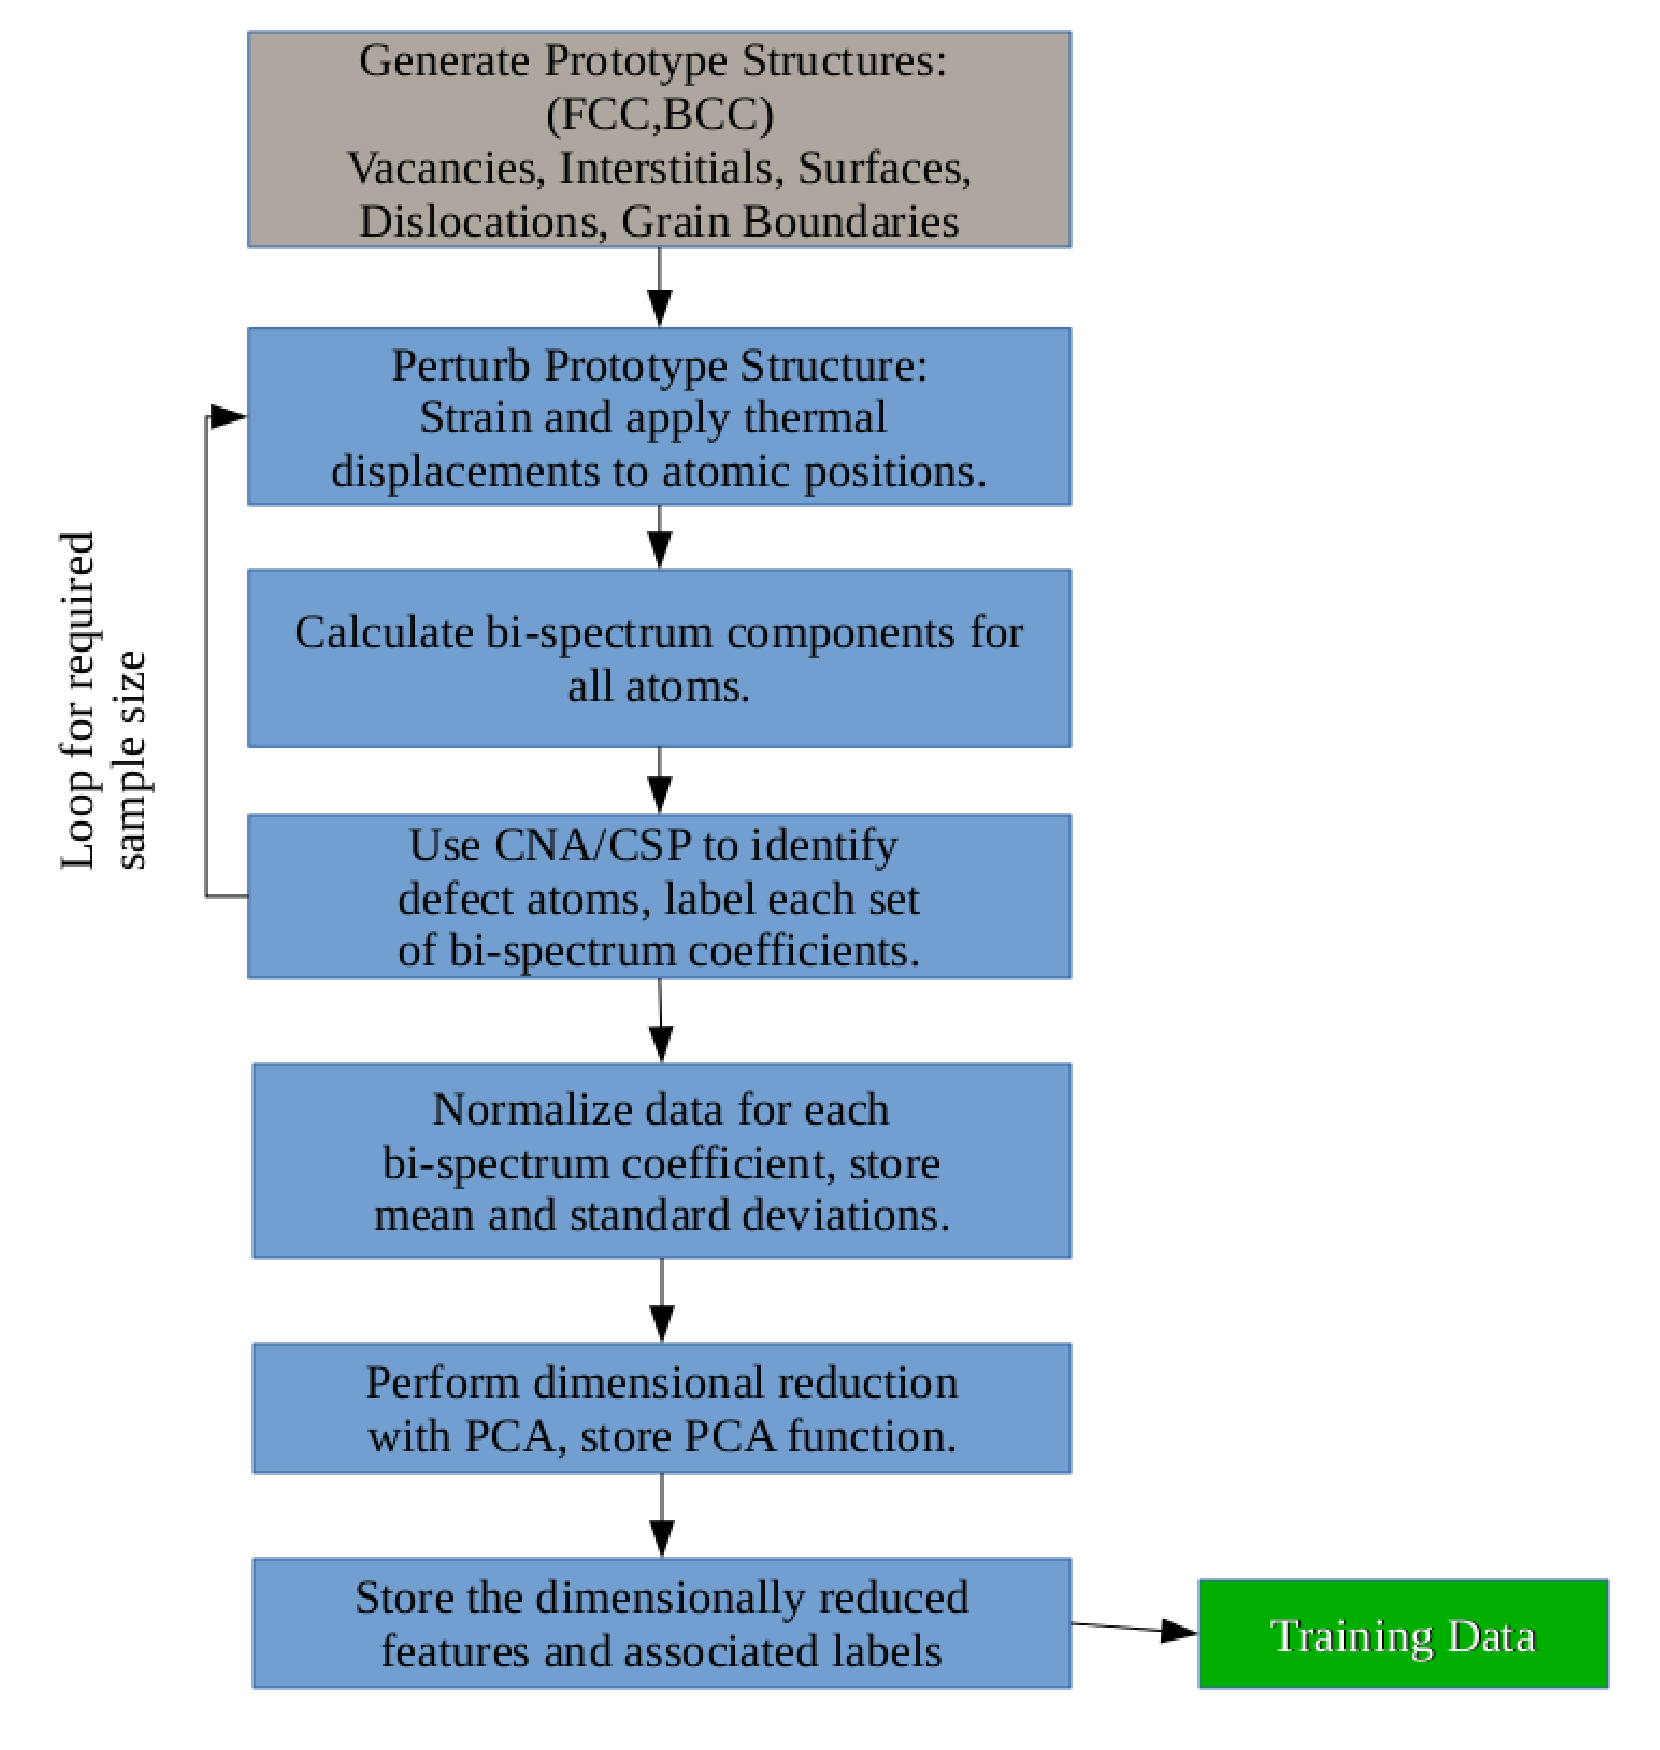
\includegraphics[scale=0.5]{Figures/cropped_feature_gen.eps}
    \rule{35em}{0.5pt}
  \caption[]{Algorithm for building the training data in defect identification.}
  \label{fig:training}
\end{figure}

The training process is featured schematically in \ref{fig:training}. Each cell was generated as a prototype structure (before any strains or thermal perturbations), after which the defects were initially identified by use of either Common Neighbor Analysis (CNA)\cite{Stukowski2012} or Centrosymmetry Paramter (CSP)\cite{Kelchner1998}. The full description of each prototype training cell is included in Appendix \ref{AppendixA}. CNA was used to capture the bulk regions of the crystals, since an individual defect was present in each prototype structure, then the non-bulk atoms could be labeled with their proper class for each case. CSP was used in cases where only minor perturbations needed to be considered as part of the defect, such as for full-dislocation core atoms. 

Each prototype was perturbed through strain and small random variations to simulate temperature fluctuations, then the bi-spectrum components were computed for each atom using a dynamic library in the LAMMPS \cite{Plimpton1995} code. The set of all bispectrum coefficients were then stored, along with each atom's associated zero-temperature and strain free defect labels. This procedure was repeated for each prototype until a sufficient spectrum of perturbations was aquired for each defect. The data were then transformed to have zero mean, and were scaled by the standard deviation of each feature (bi-spectrum component) such that the magnitude difference between bi-spectrum coefficients would not affect their significance in the machine learning algorithms. The complete training data set had approximately 5 million atoms with approximately 600,000 labeled defect atoms.

\begin{figure}[htbp]
  \centering
    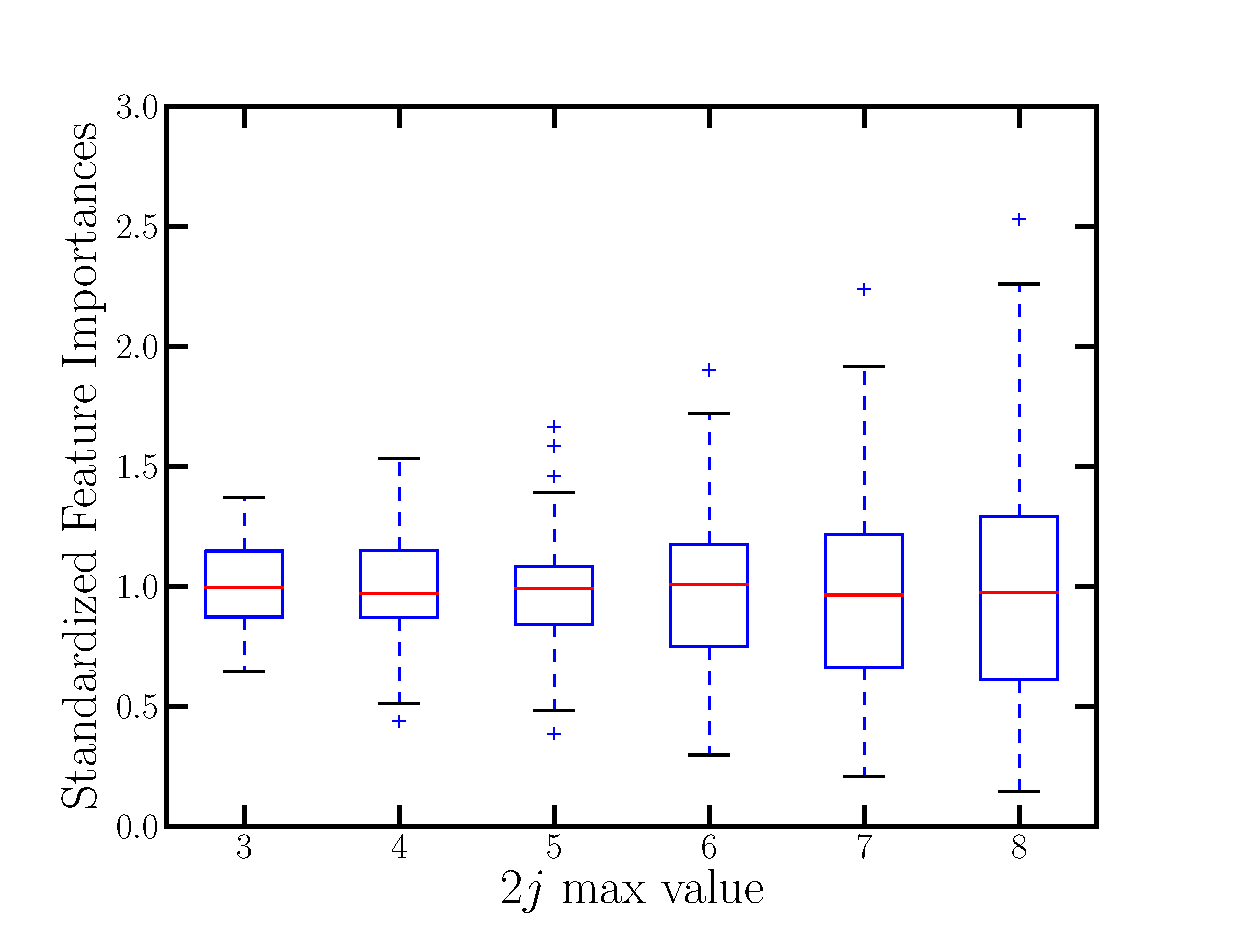
\includegraphics[scale=0.50]{Figures/featureimportance.eps}
    \rule{35em}{0.5pt}
  \caption[]{Distribution of feature importances calculated during random forest construction. The box represents the upper and lower quartile limits, with a line at the median. The whiskers show the total data range, with outliers represented by points.}
  \label{fig:featimport}
\end{figure}

Dimensionality reduction is difficult at this point, because while bi-spectrum components may provide minimal variance in the data for the currently chosen defects, these coefficients may be required to identify the specificities of new defects introduced into the data set. For this reason, we chose not to perform dimensionality reduction by means of eliminating the features which provided the least variance in classification outcome. The feature importances are implicity calculated while building random forests by determining the number of splits needed for each feature. In \ref{fig:featimport}, the feature importances are plotted as a function of $2j$, the parameter in Eqn. 2.31 that determines the limits of the bispectrum expansion. The importances have been standardized such that they each have a mean of 1. The further the values are from one, the more or less important they are to identifying defects within the crystal. As expected, as the number of bispectrum components increases the relative importances begin to spread. At $2j=8$, which gives a total of 55 bispectrum coefficients, even the least significant values are still about 10 \% as important as the mean, leading us to believe that some particular defects may require higher order bispectrum expansions. It seems there are no negligable bispectrum contributors, even with 55 coeffficients.

\begin{figure}[htbp]
  \centering
    \includegraphics[scale=0.5]{Figures/full_PCA.eps}
    \rule{35em}{0.5pt}
  \caption[]{Two component PCA decpomposition of all defects considered in this study.}
  \label{fig:PCA}
\end{figure}

As an investigative tool into the efficacy of using the bi-spectrum coefficients for defect features, we performed a principal component analysis on the $2j=8$ data sets, with 55 total features. The PCA was performed, and only the first two principal components were considered for the visualization shown in Fig.\ref{fig:PCA}. It becomes immediately apparant that more than two components are required to uniquely identify the defects considered in this study. There is substantial overlap between defect regions which causes missed or erroneous classifications. The most relevant finding from the PCA in Figs. \ref{fig:PCA} and \ref{fig:surfPCA} is that small atomic position perturbations from strain or temperature will produce closely clustered (in terms of eucledian distance) points in bi-spectrum space. This means that using bispectrum coefficients as features will be a stable methodology for nearest neighbor or descision tree algorithms.

The spread in the PCA distribution for each defect results from the thermal and stress-based position fluctuations relative to each atom's nearest neighbors. It's interesting to note that a few defects have dense distributions relative to the bulk atom distributions, including the FCC vacancies, FCC full dislocations, and BCC tetrahedal interstitial sites. This implies that these defects have environments which are less suseptable to variation under thermal fluctuations when compared to bulk sites. A second plot of the defect PCA decomposition, with only bulk and surface defects is shown in Fig. \ref{fig:surfPCA}. Even in this low dimensional representation, it can be seen that the different surface defects tend to separate in bi-spectrum coefficient space such that a dividing surface can be defined between bulk and defective regions. These encouraging results lead us to push foreward with the technique's implementation.

\begin{figure}[htbp]
  \centering
    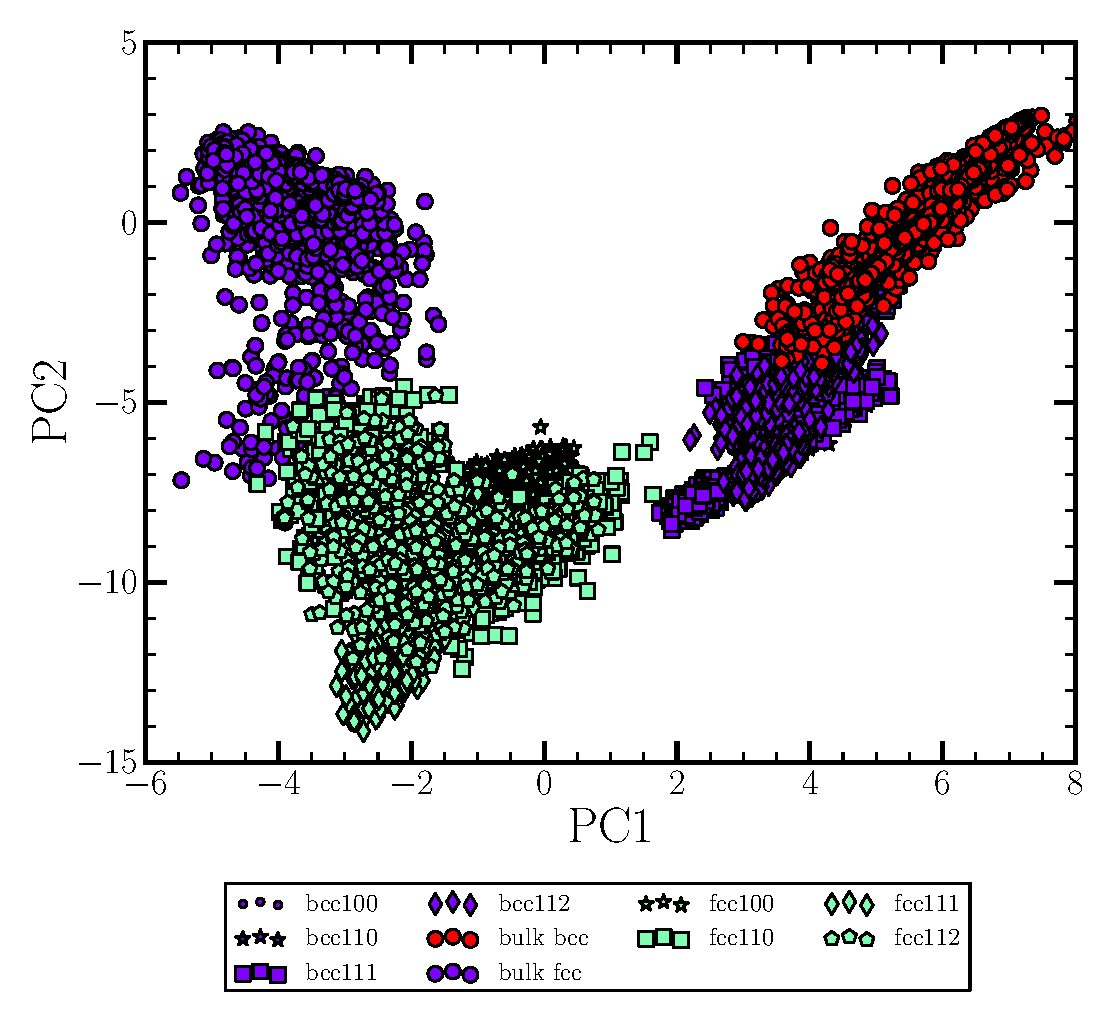
\includegraphics[scale=0.5]{Figures/surfacePCA.eps}
    \rule{35em}{0.5pt}
  \caption[]{Two component PCA decpomposition for only surface defects and bulk atoms in FCC and BCC.}
  \label{fig:surfPCA}
\end{figure}

\subsection{Algorithm Training and Optimization}

Both a nearest neighbors (NN) and random forest ensemble (RF) algorithm were trained with the bispectrum data for different maximum $2j$ values to evaluate performance of the bispectrum generation as a function of training set accuracy. Our final training data set resulted in 21 different labeled catagories. Since some catagories had significantly more members then others (bulk fcc, bcc for instance), we chose to evenly sample from each catagory to generate the final data which the algorithms were trained on. The timing and performance results for different numbers of bispectrum coefficients is shown in Fig. \ref{fig:performance}. The NN algorithm used $k=5$ nearest neighbors, and the RF algorithm used at least 10 samples per leaf with 1000 trees in the ensemble. We see that adding bispectrum coefficients progressively increases the training set accuracy, where values beyond $2j=8$ saw dimishining returns in terms of training set accuracy. The bispectrum generation algorithm seems to scale with $O((2j)^2)$, giving an optimal value for speed and accuracy between $2j=3$ and $2j=4$.

\begin{figure}[htbp]
  \centering
    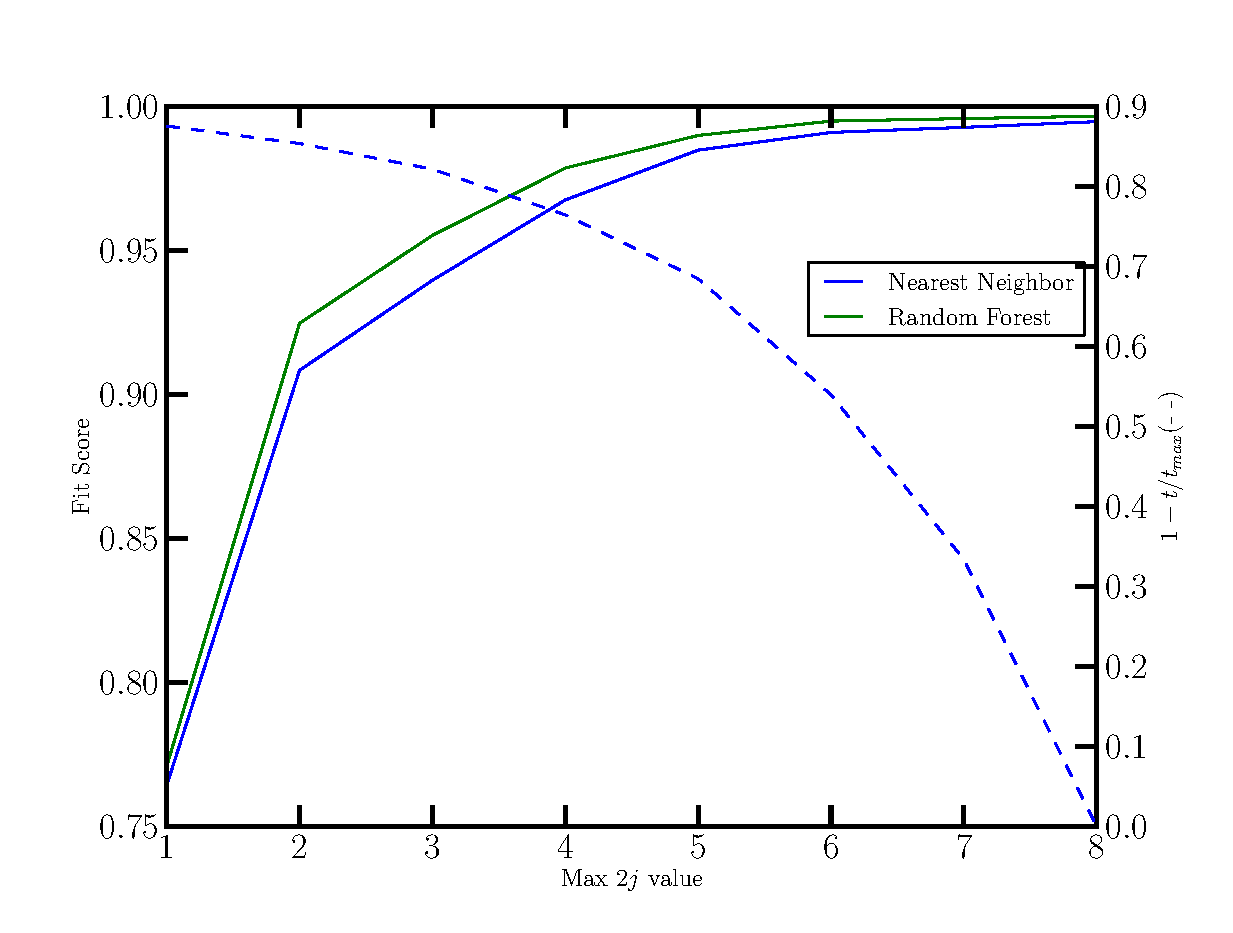
\includegraphics[scale=0.5]{Figures/performance.eps}
    \rule{35em}{0.5pt}
  \caption[]{Performance information for BiDef algorithms as a function of the maximum $2j$ value used. Timing information is given as $1-t/t_{max}$ such that 1 would be the fastest time of the $2j$ values tested. Fitted Score is a indicator of how well the training set was fit.}
  \label{fig:performance}
\end{figure}

The way the defect identification code is currently implemented, it needs to be run as a post processing step from a LAMMPS dump file. The atomic positions are read from the LAMMPS file, and the bispectrum components are then generated in a manner similar to building the training set. The set of bispectrum coefficients must be normalizing using the same mean and standard deviation data as gathered from the training samples, so the stored values are used to normalize the current bispectrum components being evaluated. They are then predicted using either the nearest neighbor or random forest algorithm, and an object is returned which has the unique identification for each atom. These results can be visualized as shown in the next section. This algorithm is referred to from this point as BiDef, a shortening of bispectrum based machine learning for defect identification.

\begin{figure*}[htbp]
  \centering
    \subfloat[]{\label{fig:VRF}
    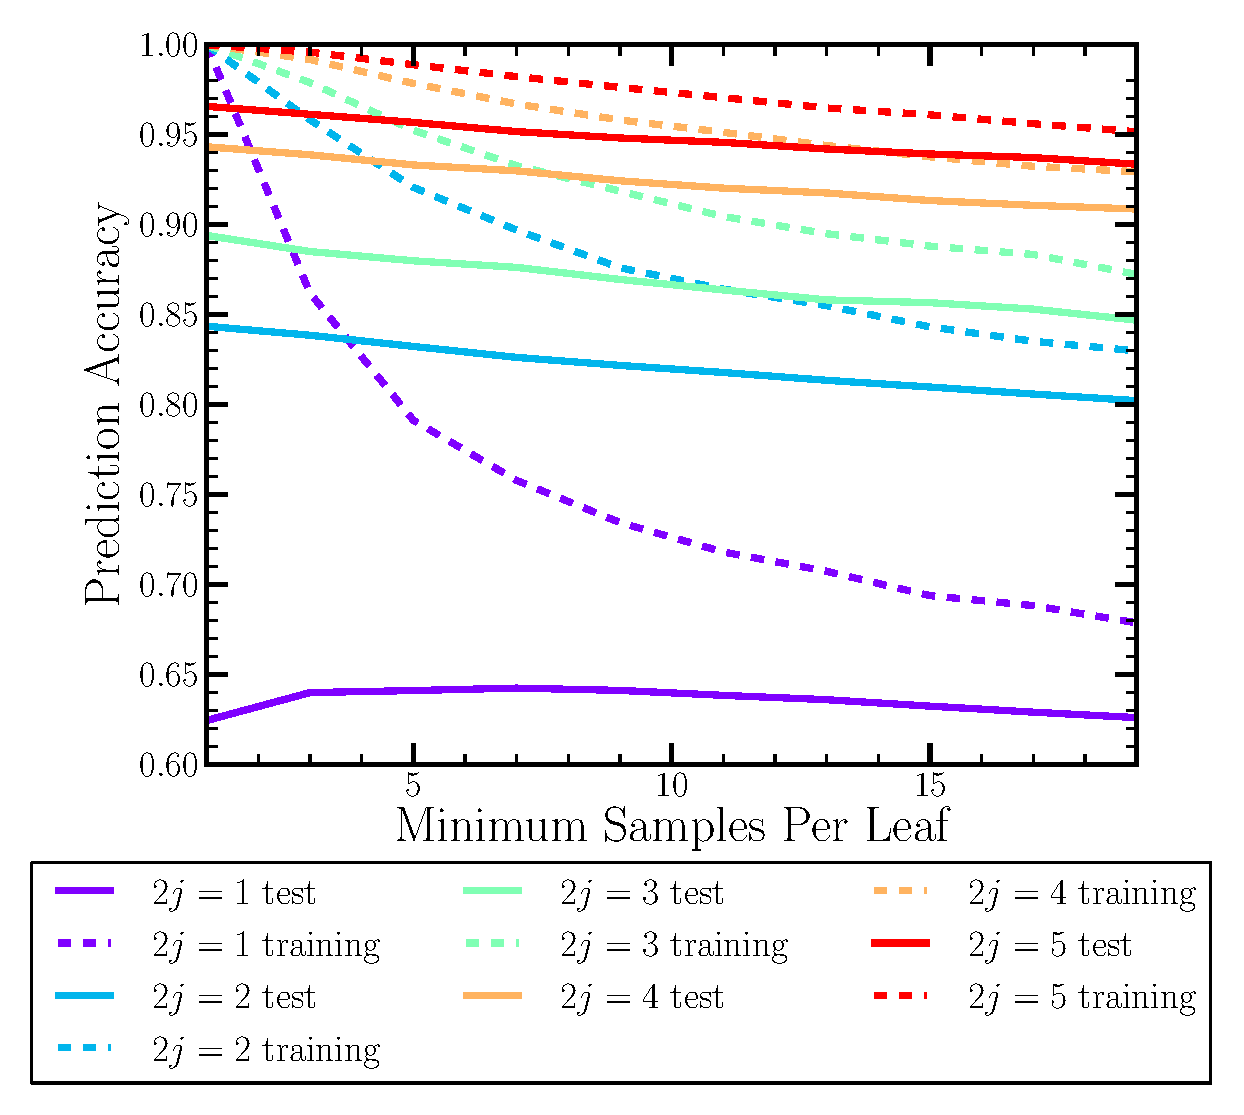
\includegraphics[scale=0.5]{Figures/Variance_RF.eps}} \\
    \subfloat[]{\label{fig:VNN}
    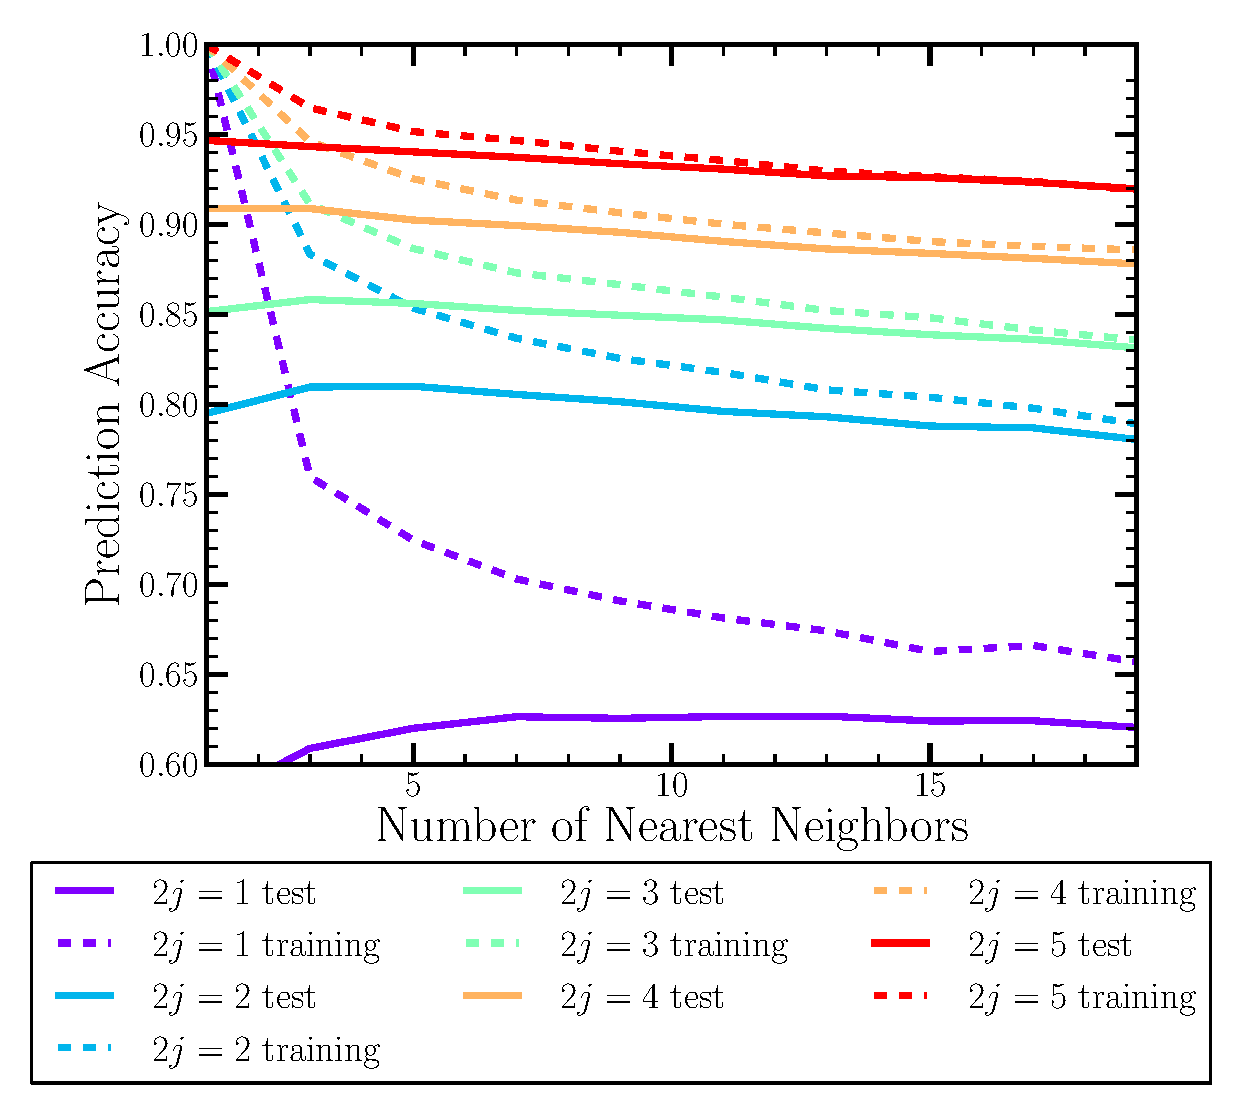
\includegraphics[scale=0.5]{Figures/Variance_NN.eps}} \\
    \rule{35em}{0.5pt}
  \caption[]{Prediction accuracy for both the training and testing set data as a function of  a)the maximum leaves per node and b) the number of nearest neighbors. The data is represented for 5 different bispectrum coeffcient cutoffs, $max2j$ values.}
  \label{fig:variance}
\end{figure}

Statistical verification methods like cross validation are quite diffucult for this algorithm since there is no objectively correct way to identify defective atoms in previously unseen data. A limited method of evaluating error is to verify correct predictions within the training data. Portions of the pre-generated training data are left out of the training procedure and then compared after training, with the left-out data referred to as the testing set. This approach is known as a bootstrapping approach to evaulate error. The model is trained repeatedly on random samples from the total training set, and the error is evaluated for both the training set and the testing set. These two sets  The errors are averaged as the model parameters are varied to find globally optimal model parameters. The model accuracy is calulated as the fraction of correctly identified samples, the error can then be viewed as $1-accuracy$.

The results of the bootstrapping test are shown in Fig.\ref{fig:variance}. As expected, the training data prediction accuracy decreases with both increasing number of neighbors and minimum samples per leaf node. The models are overfit when few neighbors are used, or when a small number of samples per leaf node is required. Fig.\ref{fig:variance} shows the results for $2j$ values from 1 to 5, which gave the model 2 and 20 features to work with respectively. Increased numbers of bispectrum coefficients give both models greater prediction accuracy.

Interestingly for the bootstrapped accuracy of the test data set, the accuracy monotonically decreases with increased numbers of nearest nieghbors or samples per leaf. We had expected to see a maximum, followed by a decrease in accuracy caused by over-simplification in the models at high numbers of nearest neighbors or leaf-node members. We think that this behavior is due to the tight clustering and relative uniqueness of the defects in feature space. The defects in bispectrum space are so tighly clusetered that we are essentially fitting the model to 21 different points in feature space. Since we don't have any untrained defects which fall in the 'spectrum' between two other defects, the generalization, or the bias, in the model is not too important for our application.

\section{Results and Discussion}

A qualitative comparision between CSP, CNA and bispectrum with random forests defect identification algorithms is shown in Fig. \ref{fig:bcc_structures}. The results are shown for a 1-d, square nano-wire of BCC iron, which was subjected to a tensile test in a direction normal to the plane of the page (along the nanowire axis). A Nosé-Hoover thermostat \cite{Hoover1985,Nose1984} was used to control the temperature at 300K during the tensile test. ⁠A Finnis–Sinclair EAM potential\cite{Mendelev2003} was used for the iron interactions. The crystals were oriented such that the free surfaces were of the $<100>$ type, and the crystal was strained along the $[001]$ axis. The sample images are taken just as the yield (slip) process started. It's important to note that none of the atoms in this tensile test were used in traning the machine learning algorithm, the algorithm made all classifications based on previous data of a different geometry and size scale, as detailed in Appendix \ref{AppendixA}. The most obvious difference between the machine learning algorithm, \ref{fig:bidefbcc}, and the CSP/CNA algorithms is that the defects are specified. In \ref{fig:bidefbcc} we see that the surfaces are primarily $<100>$ type surfaces (dark blue), as expected from the starting cell configuration, with the other two methods the only obtainable information is that the atoms along the surface are defective relative to the bulk. Along the surfaces where the $b=\frac{a_0}{2}<111>$ dislocations leave the bulk, the surface atoms have shifted such that they are identified as $(112)$ surfaces, indicating surface slip relative to the other surface sites. The corner atoms are identifed as $(111)$ surfaces, which isn't physically accurate, but indicates that the algorithm is sensitive to the reduction in coordination. It was not trained to identify anomolies beyond simple flat surfaces, so this misidentification is to be expected at this stage. A desireable quality of the machine learning algorithm is that it is evidentally resiliant to noise in defect identification. When comparing the machine learned algorithm to \ref{fig:cspbcc} or \ref{fig:cnabcc}, we can see that many of the interior atoms, particularly with the CSP algorithm, are identified as defects. In reality these atoms are simply ocillating around the lattice minima due to thermal vibrations and local variations in strain, but both CNA and CSP algorithms have mis-identified many atoms.

\begin{figure*}
\begin{center}
\subfloat[]{\label{fig:bidefbcc}
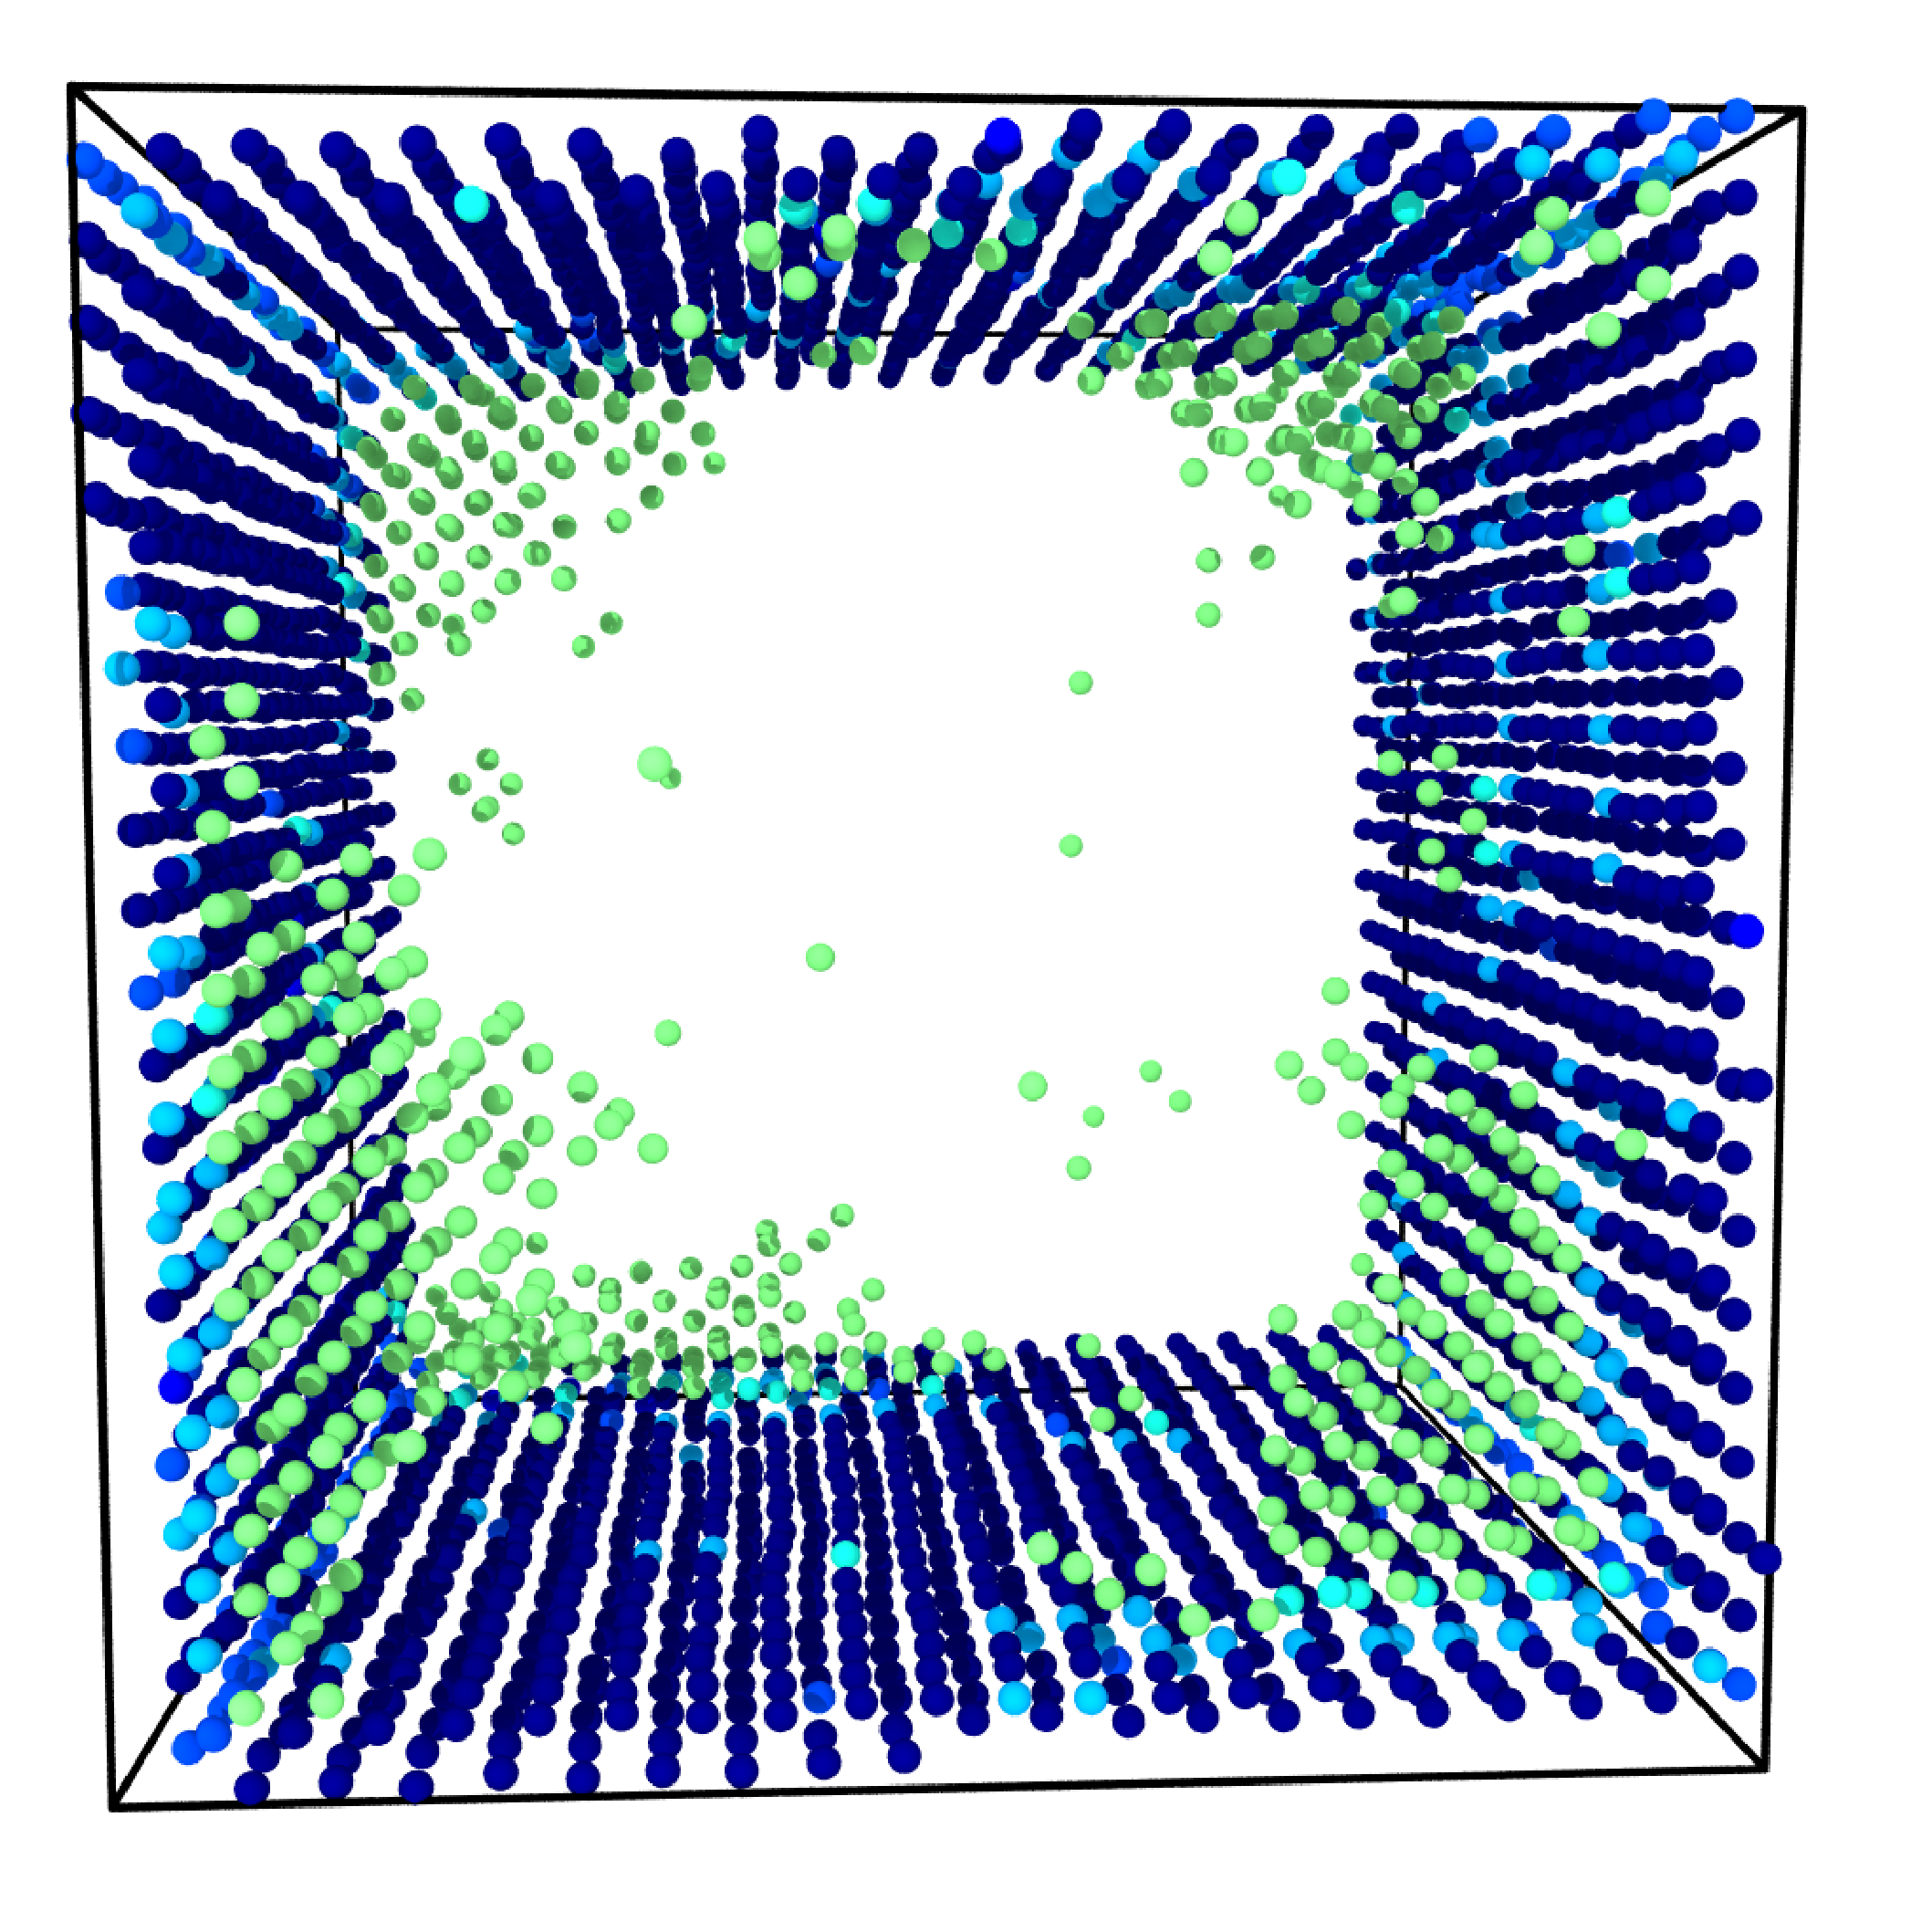
\includegraphics[width=7cm]{Figures/BCC_300_BiDef.png.eps}} \\
\subfloat[]{\label{fig:cspbcc}
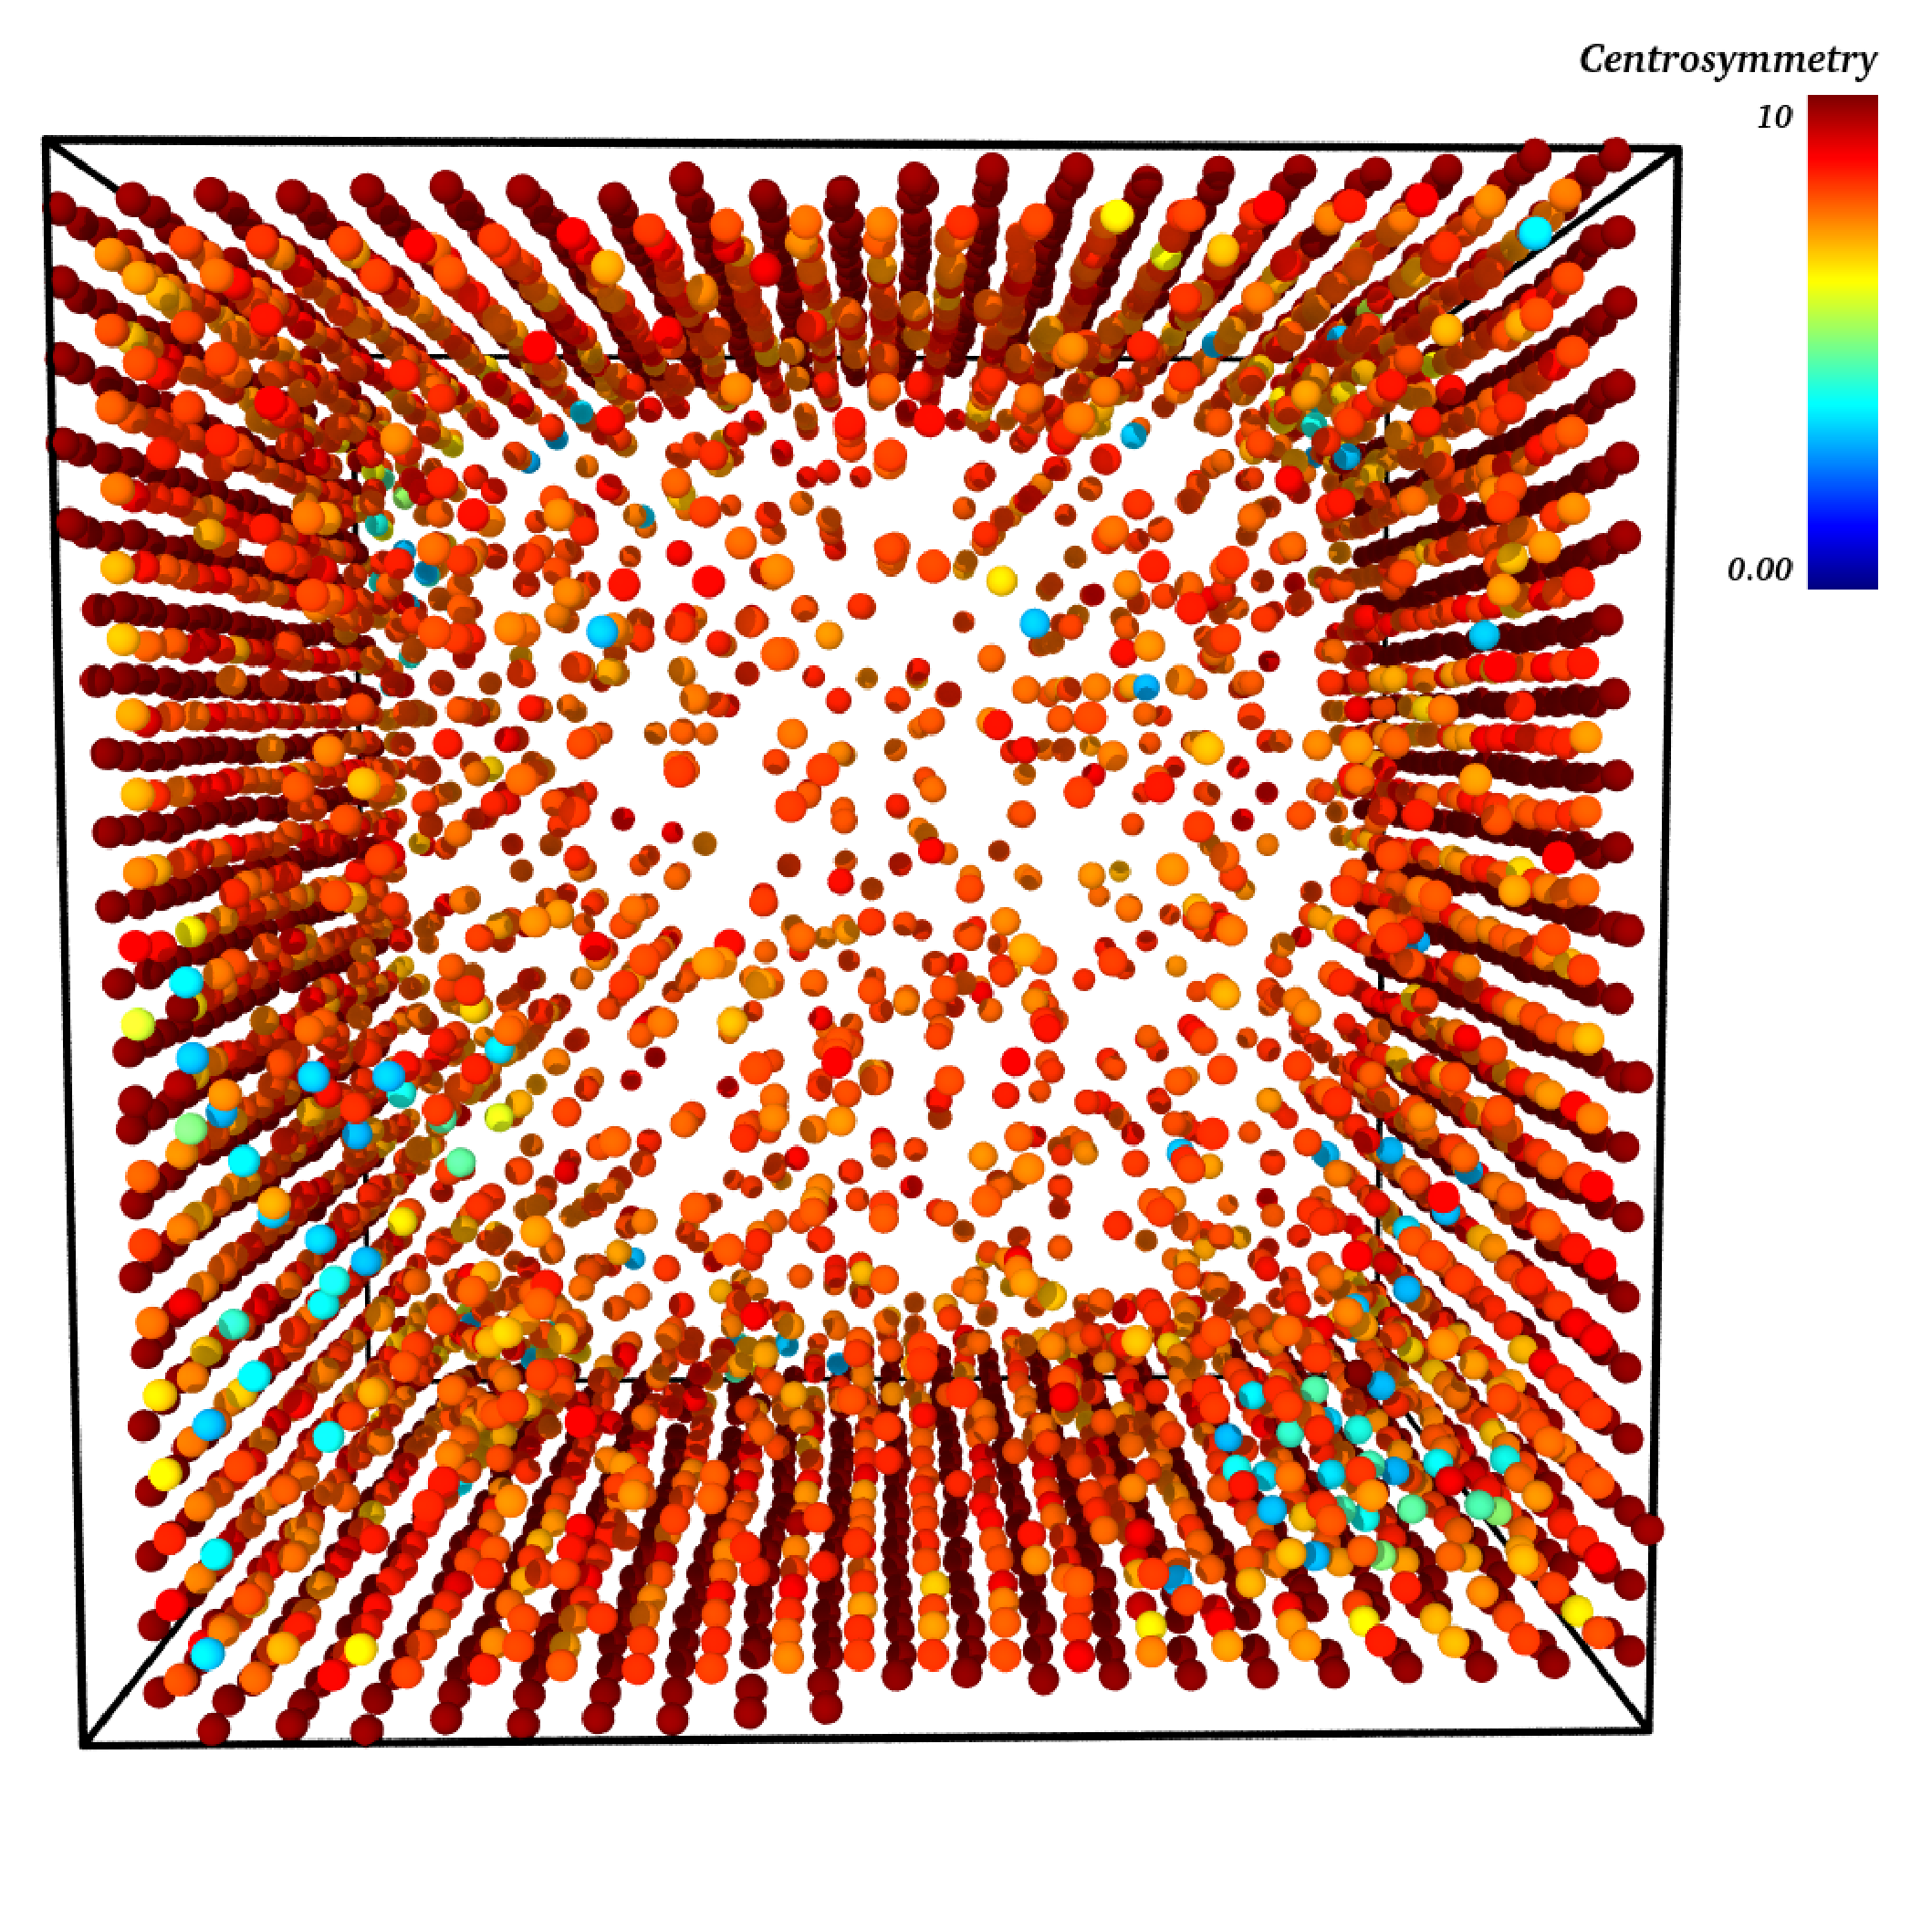
\includegraphics[width=7cm]{Figures/BCC_300_CSP.png.eps}}
\subfloat[]{\label{fig:cnabcc}
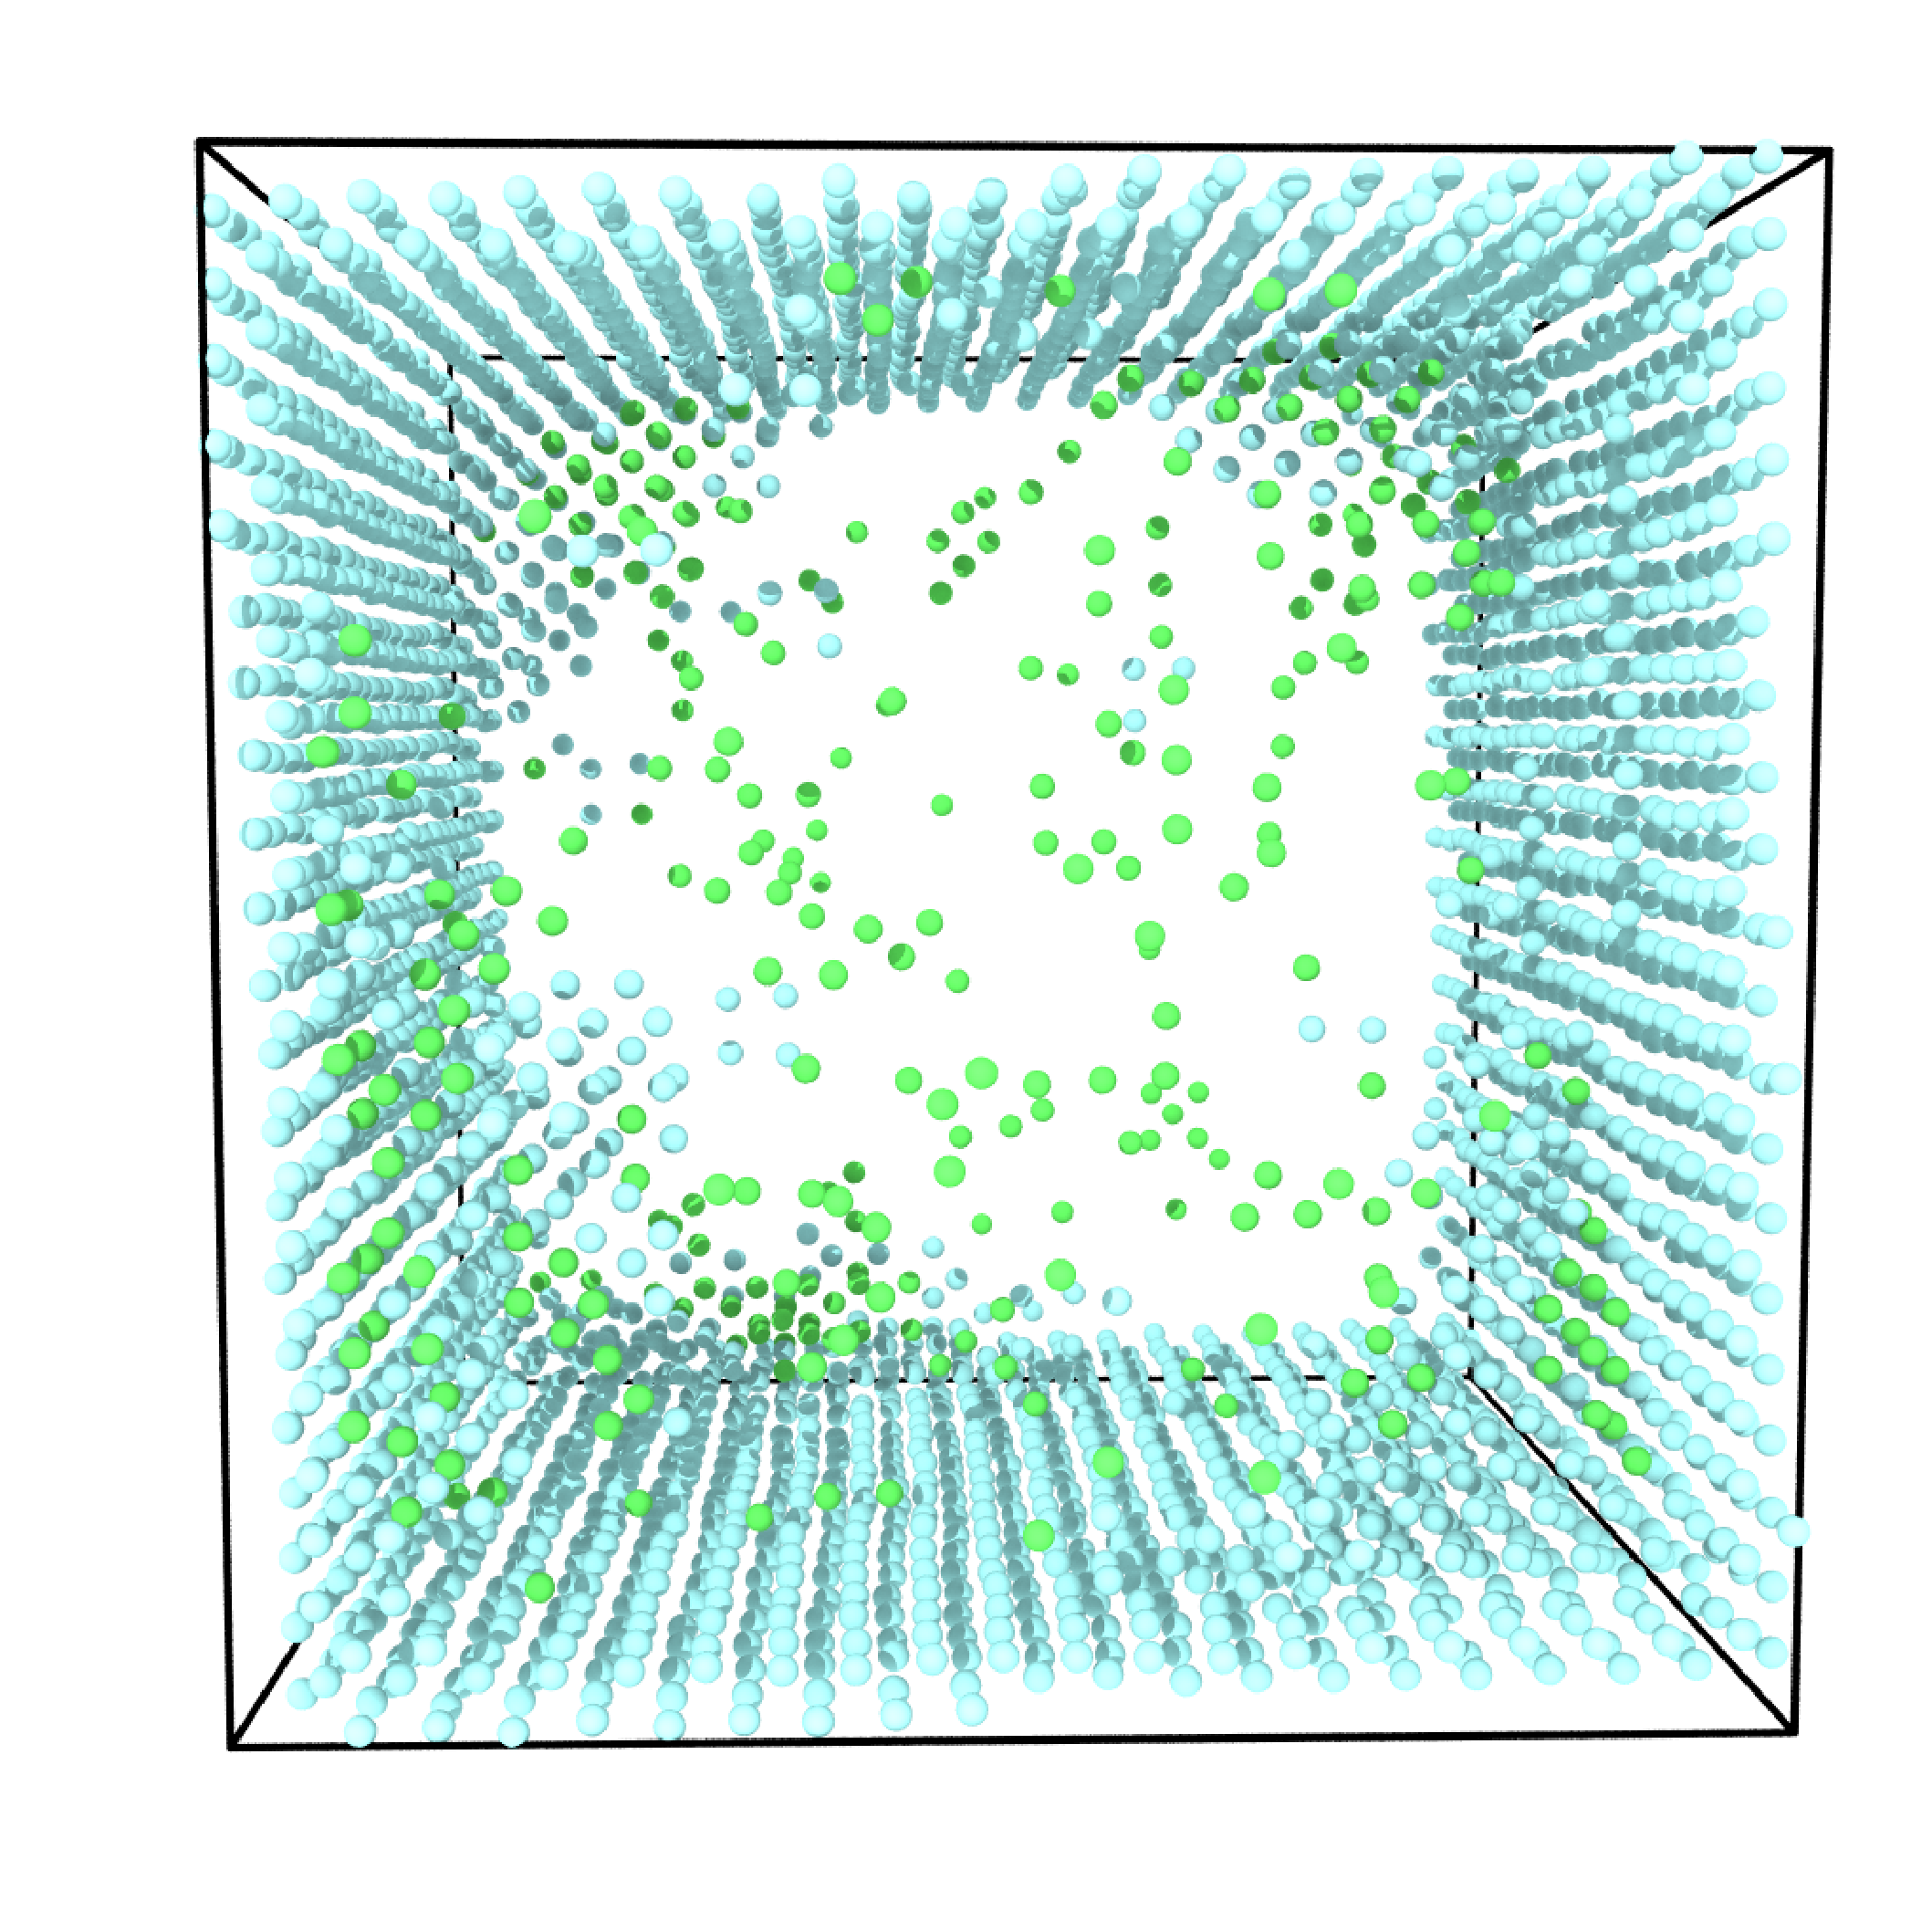
\includegraphics[width=7cm]{Figures/BCC_300_CNA.png.eps}}
\caption{Example structure of tensile-strain test yeilding in BCC iron. a) Bispectrum coefficient based method, green atoms are full-bcc dislocations, dark blue are (100) bcc surfaces, medium-blue (atoms along corners) are identified as (111) bcc atoms, and the light blue atoms are (112) bcc surface atoms. b) Same cell color coded by CSP, with all atoms where CSP $<$ 3 are removed. c) CNA colored cell, where green atoms are FCC sites, light blue atoms are unidentified sites, and all BCC atoms have been removed.}
\label{fig:bcc_structures}
\end{center}
\end{figure*}

In terms of the structure of the slipped regions in \ref{fig:bcc_structures}, some clear planes can be identified as slipped regions in the CNA and machine learned algorithm. The CSP has too much noise near the surfaces to determine where the slipped planes are located. One difficulty in identifying defects within BCC crystals is that CNA is unable to differentiate slipped regions with any specific description. In FCC systems, leading partial dislocations will leave behind HCP slip systems, which gives CNA more utiliity in defect identification. This disadvantage is overcome with the Bb-mild algorithm as it is capable of indicating that the slipped regions are BCC dislocations. Its interesting that the DXA was unable to identify the slipped regions as dislocations, as they aren't yet fully slipped, but they were still identified by BiDef. This implies that by adding training sets with partially slipped regions (plane misalignment similar to a stacking fault), the algorithm may be sensitive enough to identify regions which are on the cusp of becoming partial dislocations. This would open the possibility of predicting where yield begins in a simulation, and assisting in a subset of atoms to be chosen for nudged elastic band calculations\cite{Henkelman2000}, for instance.

\begin{figure*}
\begin{center}
\subfloat[]{\label{fig:bidefbcc}
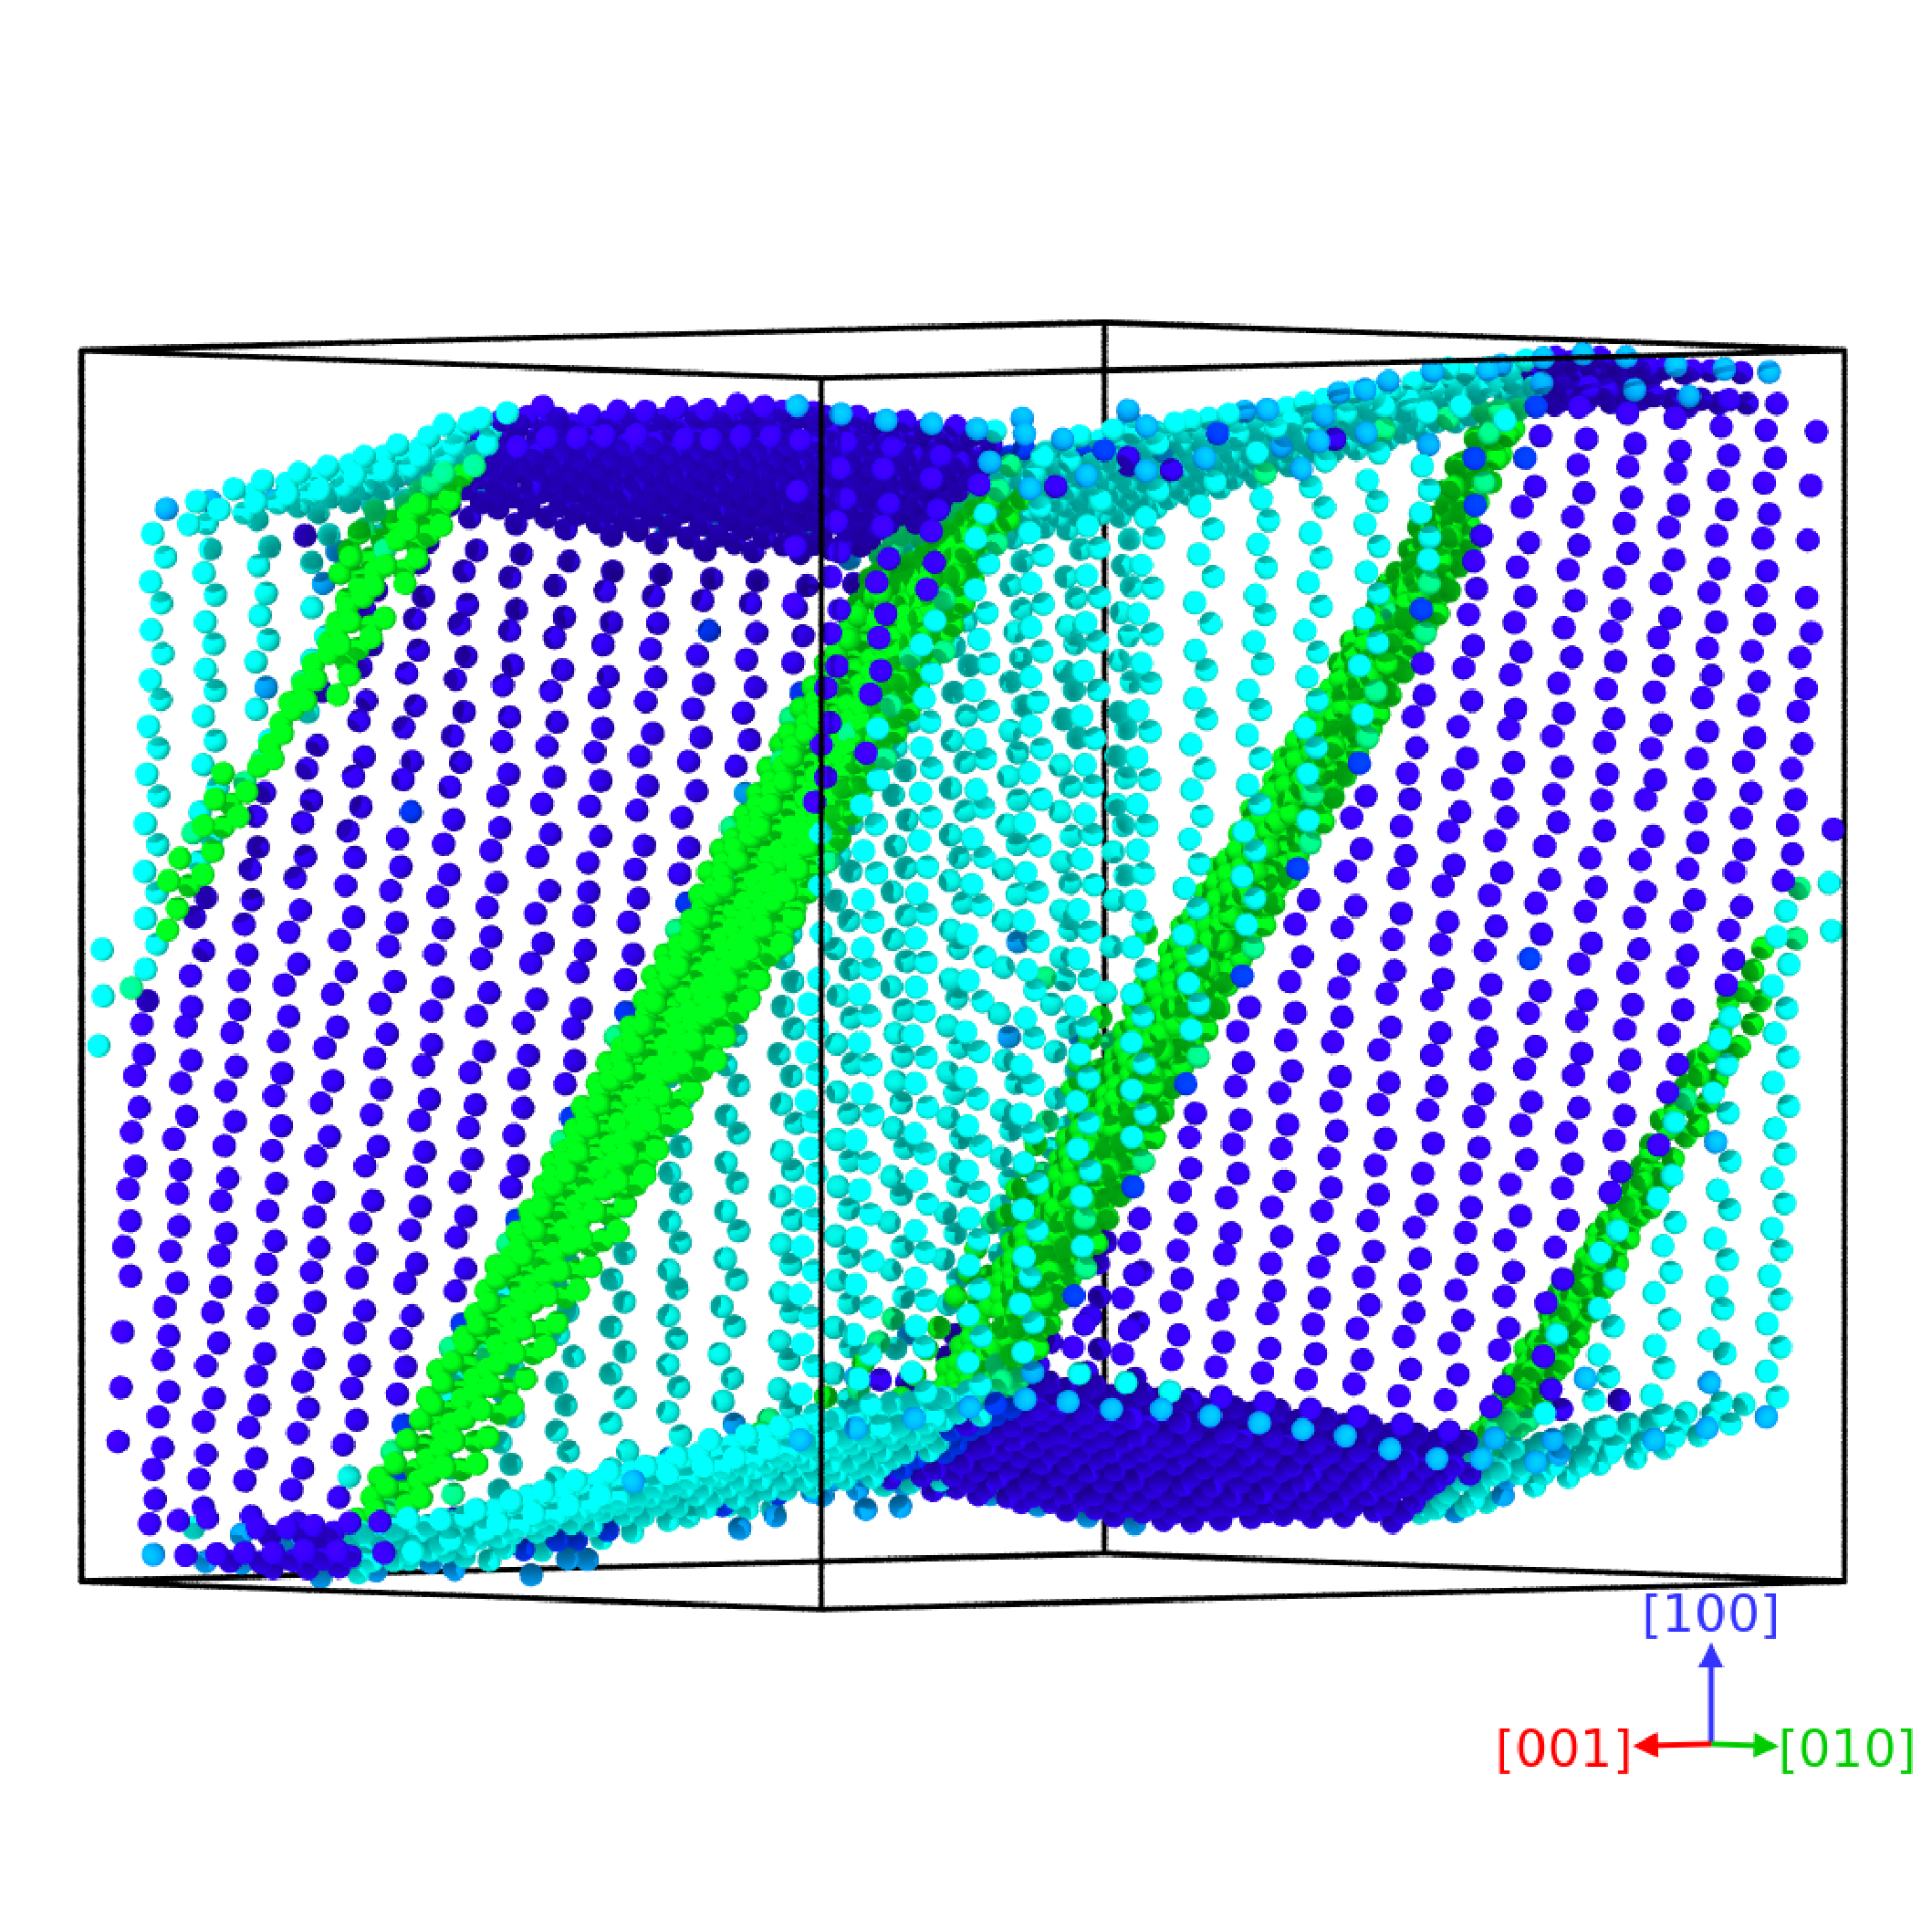
\includegraphics[width=7cm]{Figures/BCC_300_STRAIN_BiDef.png.eps}} \\
\subfloat[]{\label{fig:cspbcc}
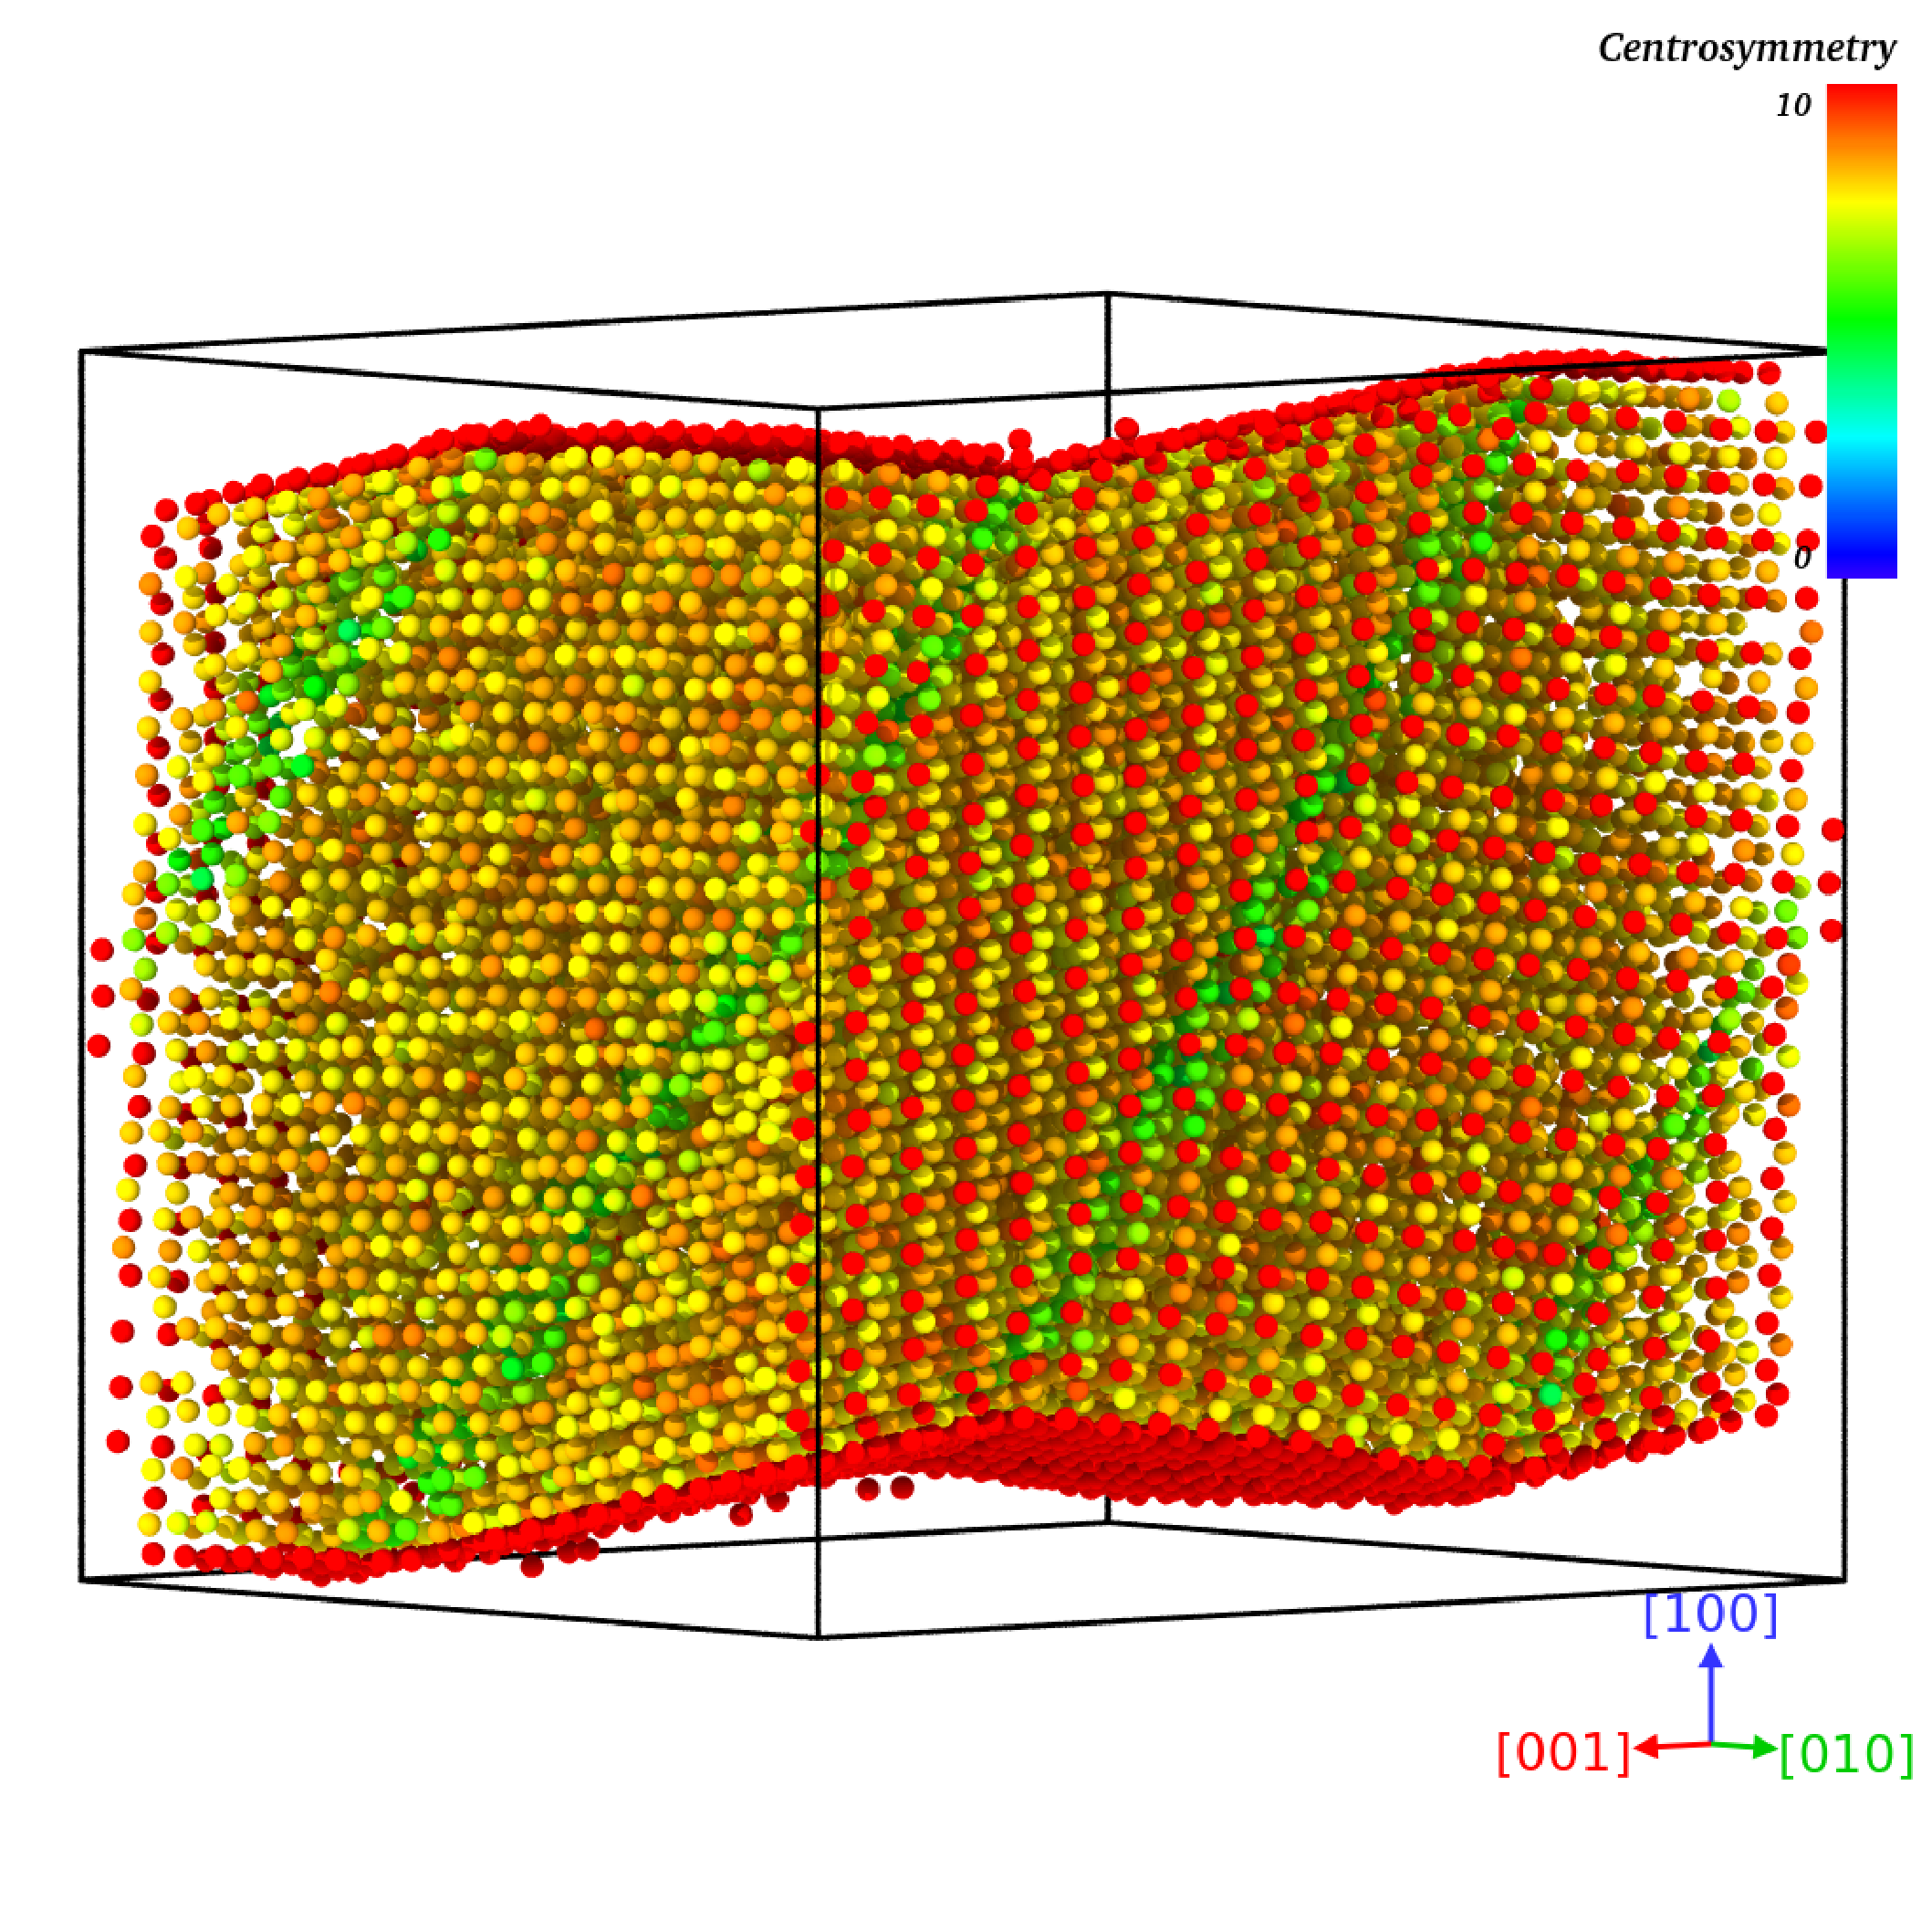
\includegraphics[width=7cm]{Figures/BCC_300_STRAIN_CSP.png.eps}}
\subfloat[]{\label{fig:cnabcc}
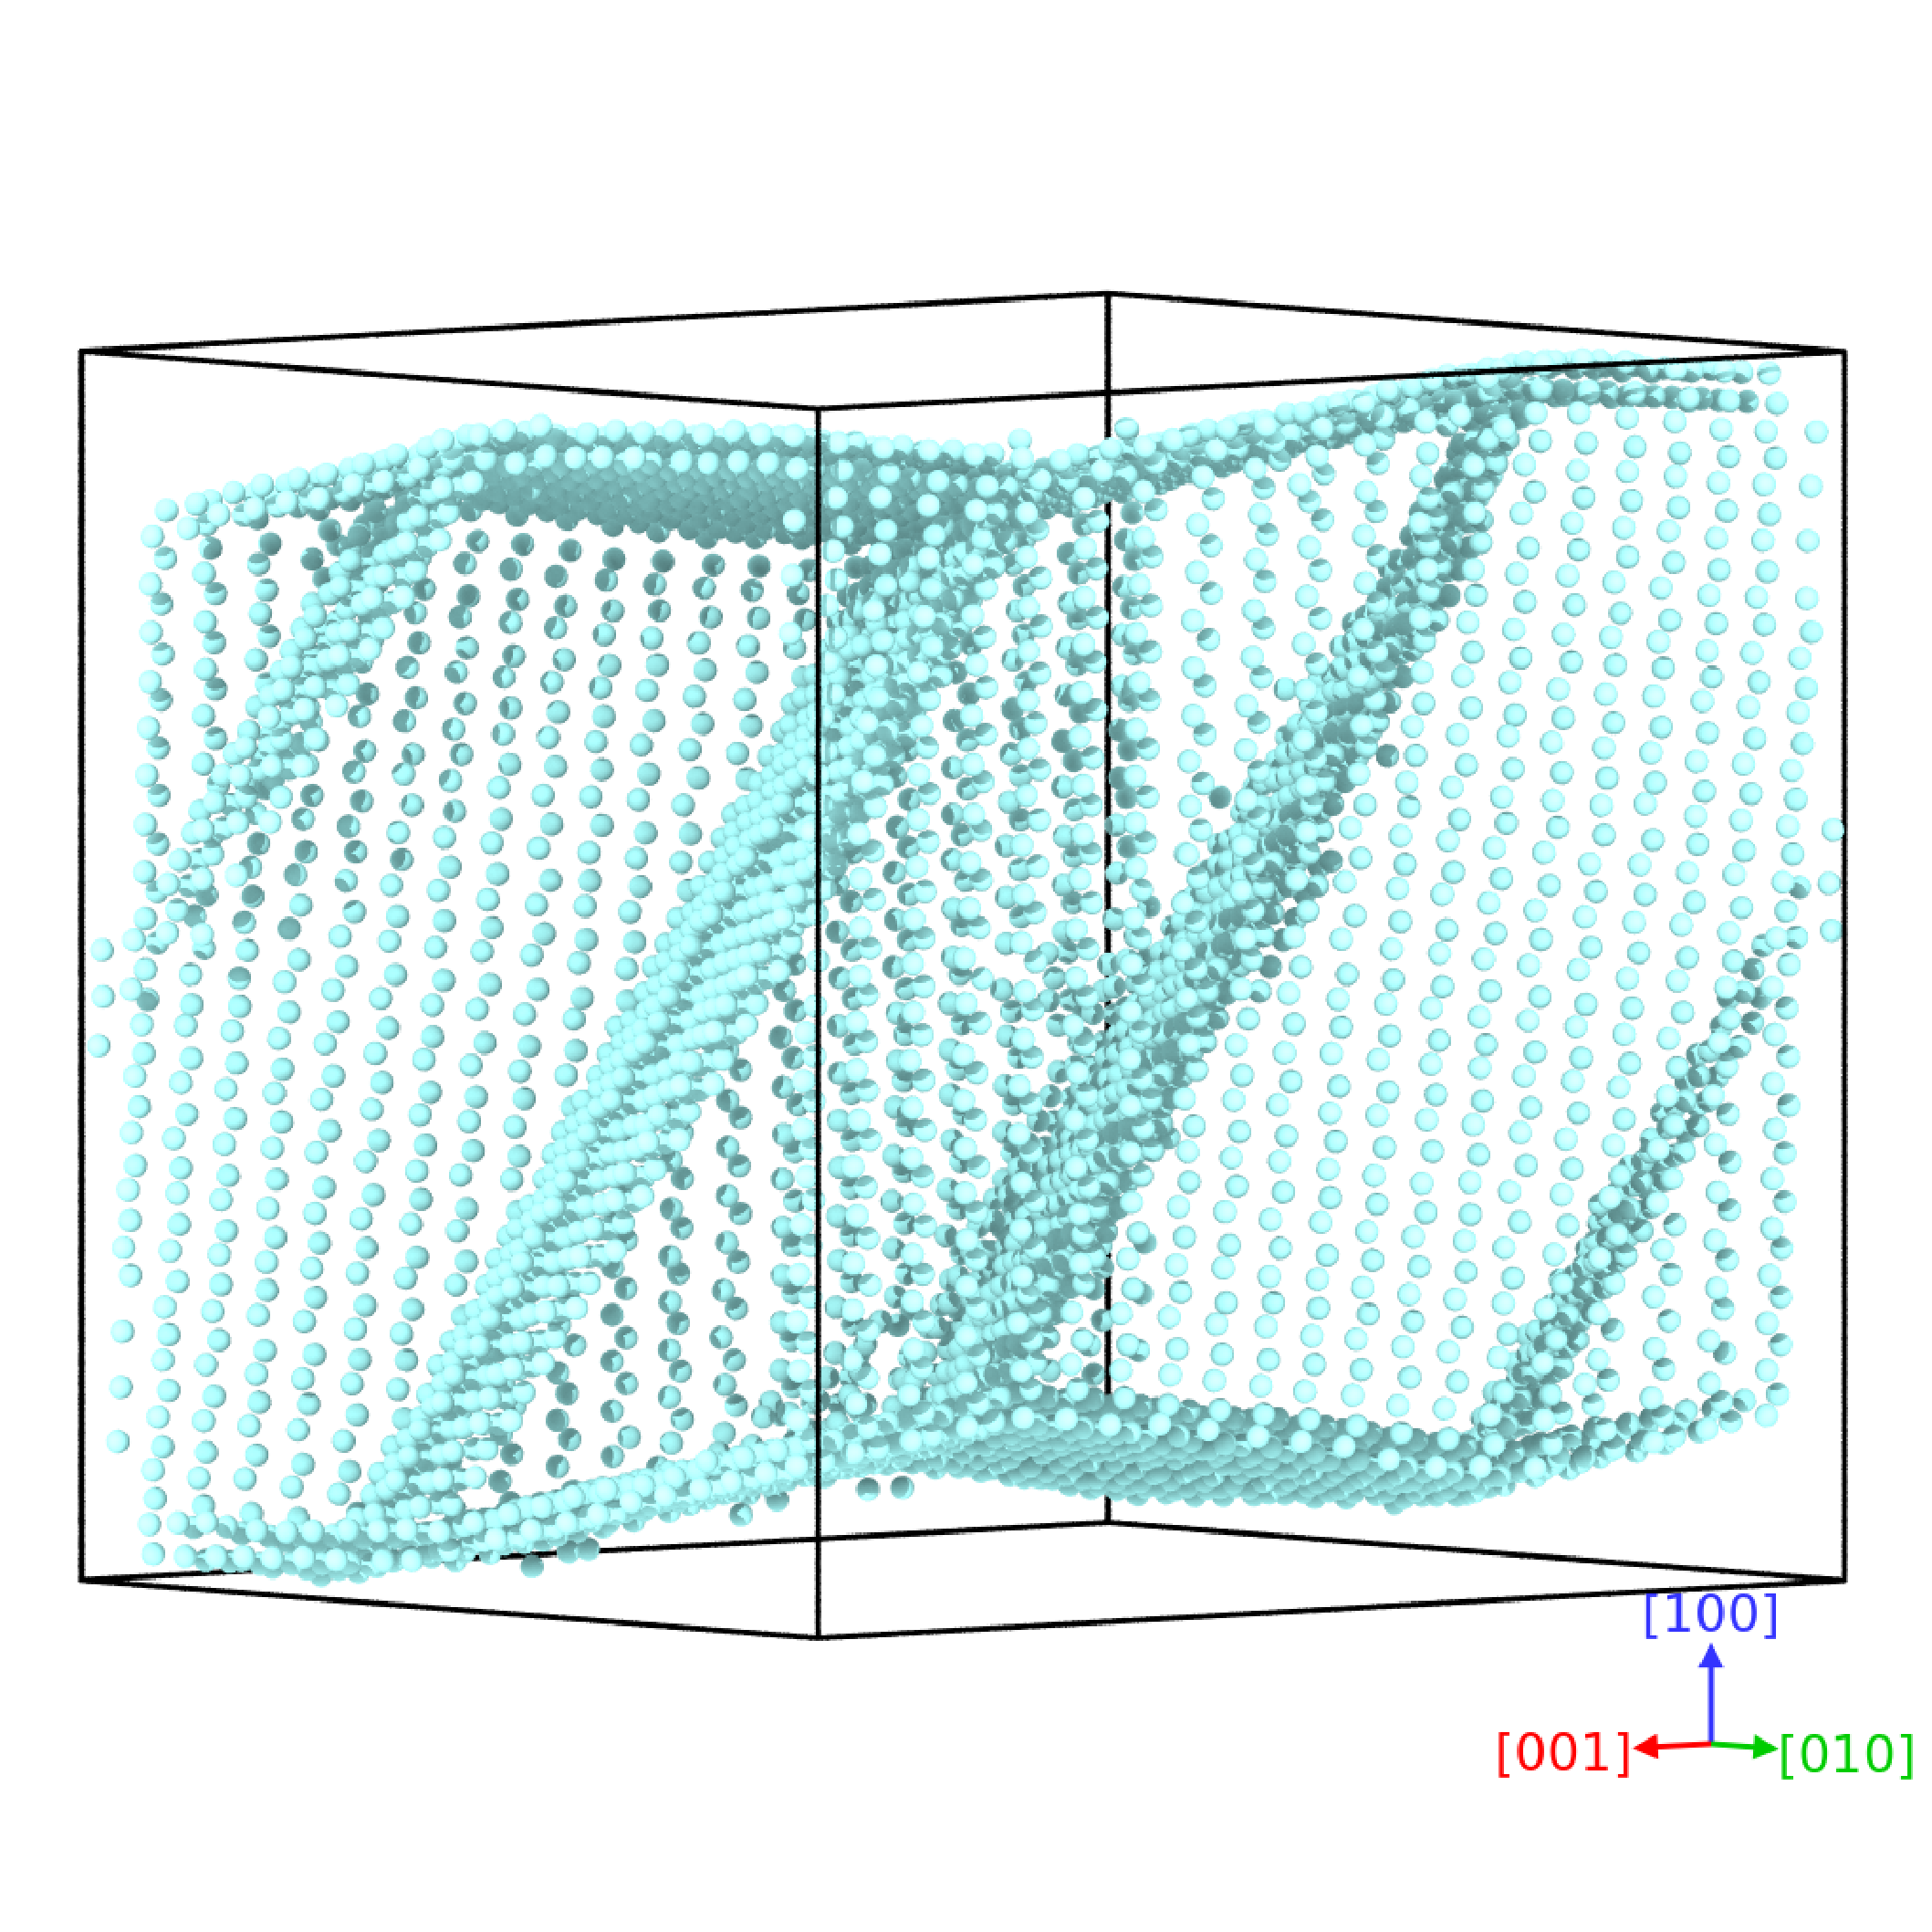
\includegraphics[width=7cm]{Figures/BCC_300_STRAIN_CNA.png.eps}}
\caption{Large-strain (10\%) structure of tensile-strain test yeilding in BCC iron. a) Bispectrum coefficient based method, green atoms are full-bcc dislocations, dark blue are (100) bcc surfaces, medium-blue (atoms along corners) are identified as (111) bcc atoms, and the light blue atoms are (112) bcc surface atoms. b) Same cell color coded by CSP, with all atoms where CSP $<$ 4.5 are removed. c) CNA colored cell, where light blue atoms are unidentified sites, and all BCC atoms have been removed.}
\label{fig:bcc_strain_structures}
\end{center}
\end{figure*}

Fig. \ref{fig:bcc_strain_structures} shows another snapshot of the same yeild stress after significant strain (10\%) has been applied. Here we see that the BiDef algorithm identified similarly defective atoms to the CNA method, however it was able to retain the proper identification of the BCC dislocations (which now cross the entire crystal). BiDef also correctly identifies that the surface atoms have switched orientation from $(100)$ to $(112)$ oriented surface atoms across the twinned boundary that forms. This information is all lost on the CNA method, as all of thes defective atoms are simply identified as "other". This figure demonstrates that the BiDef method is fairly resilient to large strains. This is expected as the algorithm was trained to incoroporate strained defects. The CSP method has a large amount of noise at large strains, while the slipped regions can still be differentiated, many of the 'bulk' atoms are misidentified as defects. 

Since the slip and surface defects in the yielding sample tests were planar in character, a useful way to charactarize noise can be to count the number of "defective" nearest neighbors to a given atom. This way atoms with two or less defective neighbors are highly unlikely to be a legitimate defect, as their presense on a plane would indicate more than two defective neighbors. We can quantify 'noise' in these samples using by using this method. A series of tensile yielding simulations were performed at different temperatures as a more quantitative evaluation of noise with the BiDef method. Both FCC and BCC cells were constructed and pulled under tensile strain rate of $10^{10} \frac{1}{sec}$. The surfaces normal to the tensile direction were left as free surfaces, giving the cell a nanowire geometry. Samples were tested at 300 K, 400 K, 500 K and 600 K using a Nosé-Hoover thermostat. The FCC sample was copper and the BCC was iron, we used the same interatomic potentials as previously indicated for these materials.

\begin{figure}[htbp]
  \centering
    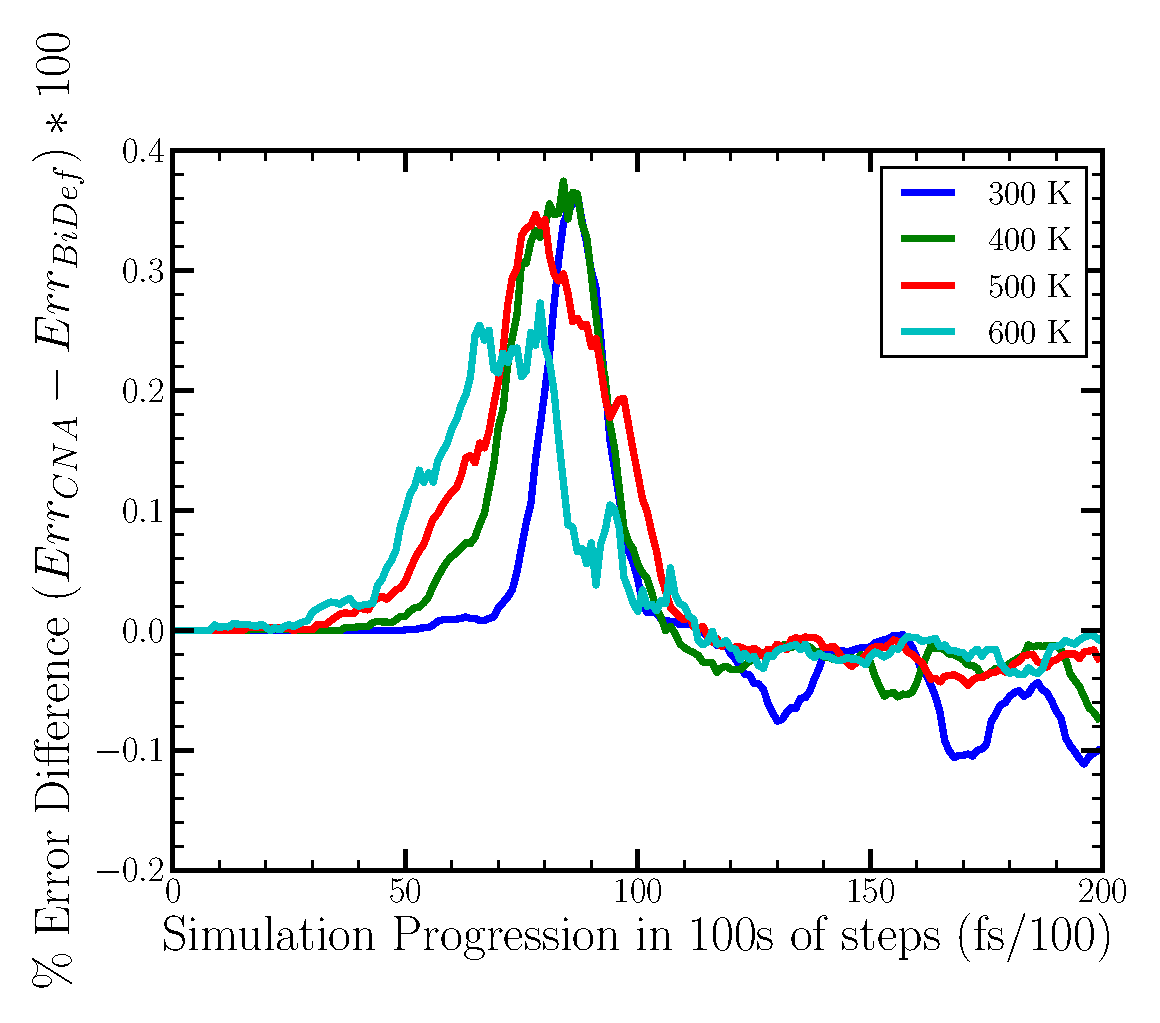
\includegraphics[scale=0.50]{Figures/bcc_error.eps}
    \rule{35em}{0.5pt}
  \caption[]{Error comparison between CNA and BiDef algorithms for different temperature tensile tests in a BCC sample.}
  \label{fig:errorbcc}
\end{figure}

\begin{figure}[htbp]
  \centering
    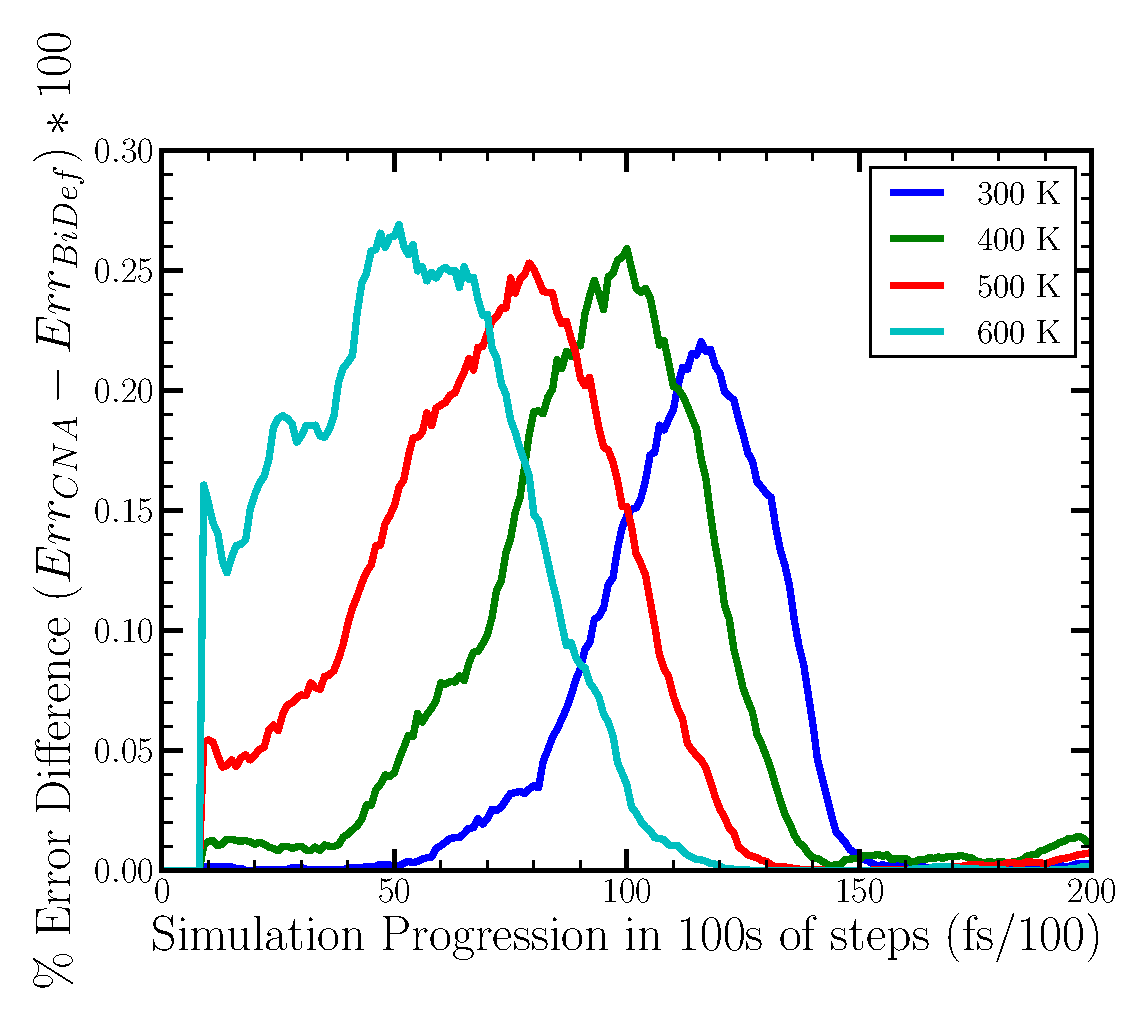
\includegraphics[scale=0.50]{Figures/fcc_error.eps}
    \rule{35em}{0.5pt}
  \caption[]{Error comparison between CNA and BiDef algorithms for different temperature tensile tests in an FCC sample.}
  \label{fig:errorfcc}
\end{figure}

Fig.\ref{fig:errorbcc} shows the error comparision between CNA and BiDef for the BCC tensile test. Portions of the curve where the error percentage is positive indicate that CNA mis-identified more defect sites than CNA, and the negative portions indicate the opposite. Prior to yielding, there is a large spike in misidentification errors in the CNA method relative to the BiDef algorithm, implying that our algorithm is more reliable at defect identification before yielding. After yielding occurs, portions of the simulation have more mislabled sites in the BiDef algorithm than in CNA. We attribute these sites to 'holes' along planes in the material, where the algorithm wasn't trained at large enough strain values for identifying BCC dislocations. From visual inspection of the simulation, the mislabled defects are almost all false-bulk assignment rather than false-defect assignments for the BiDef algorithm. Further training is likely needed for BCC defects with the BiDef method.

\begin{figure*}
\begin{center}
\subfloat[]{\label{fig:bispecnoise}
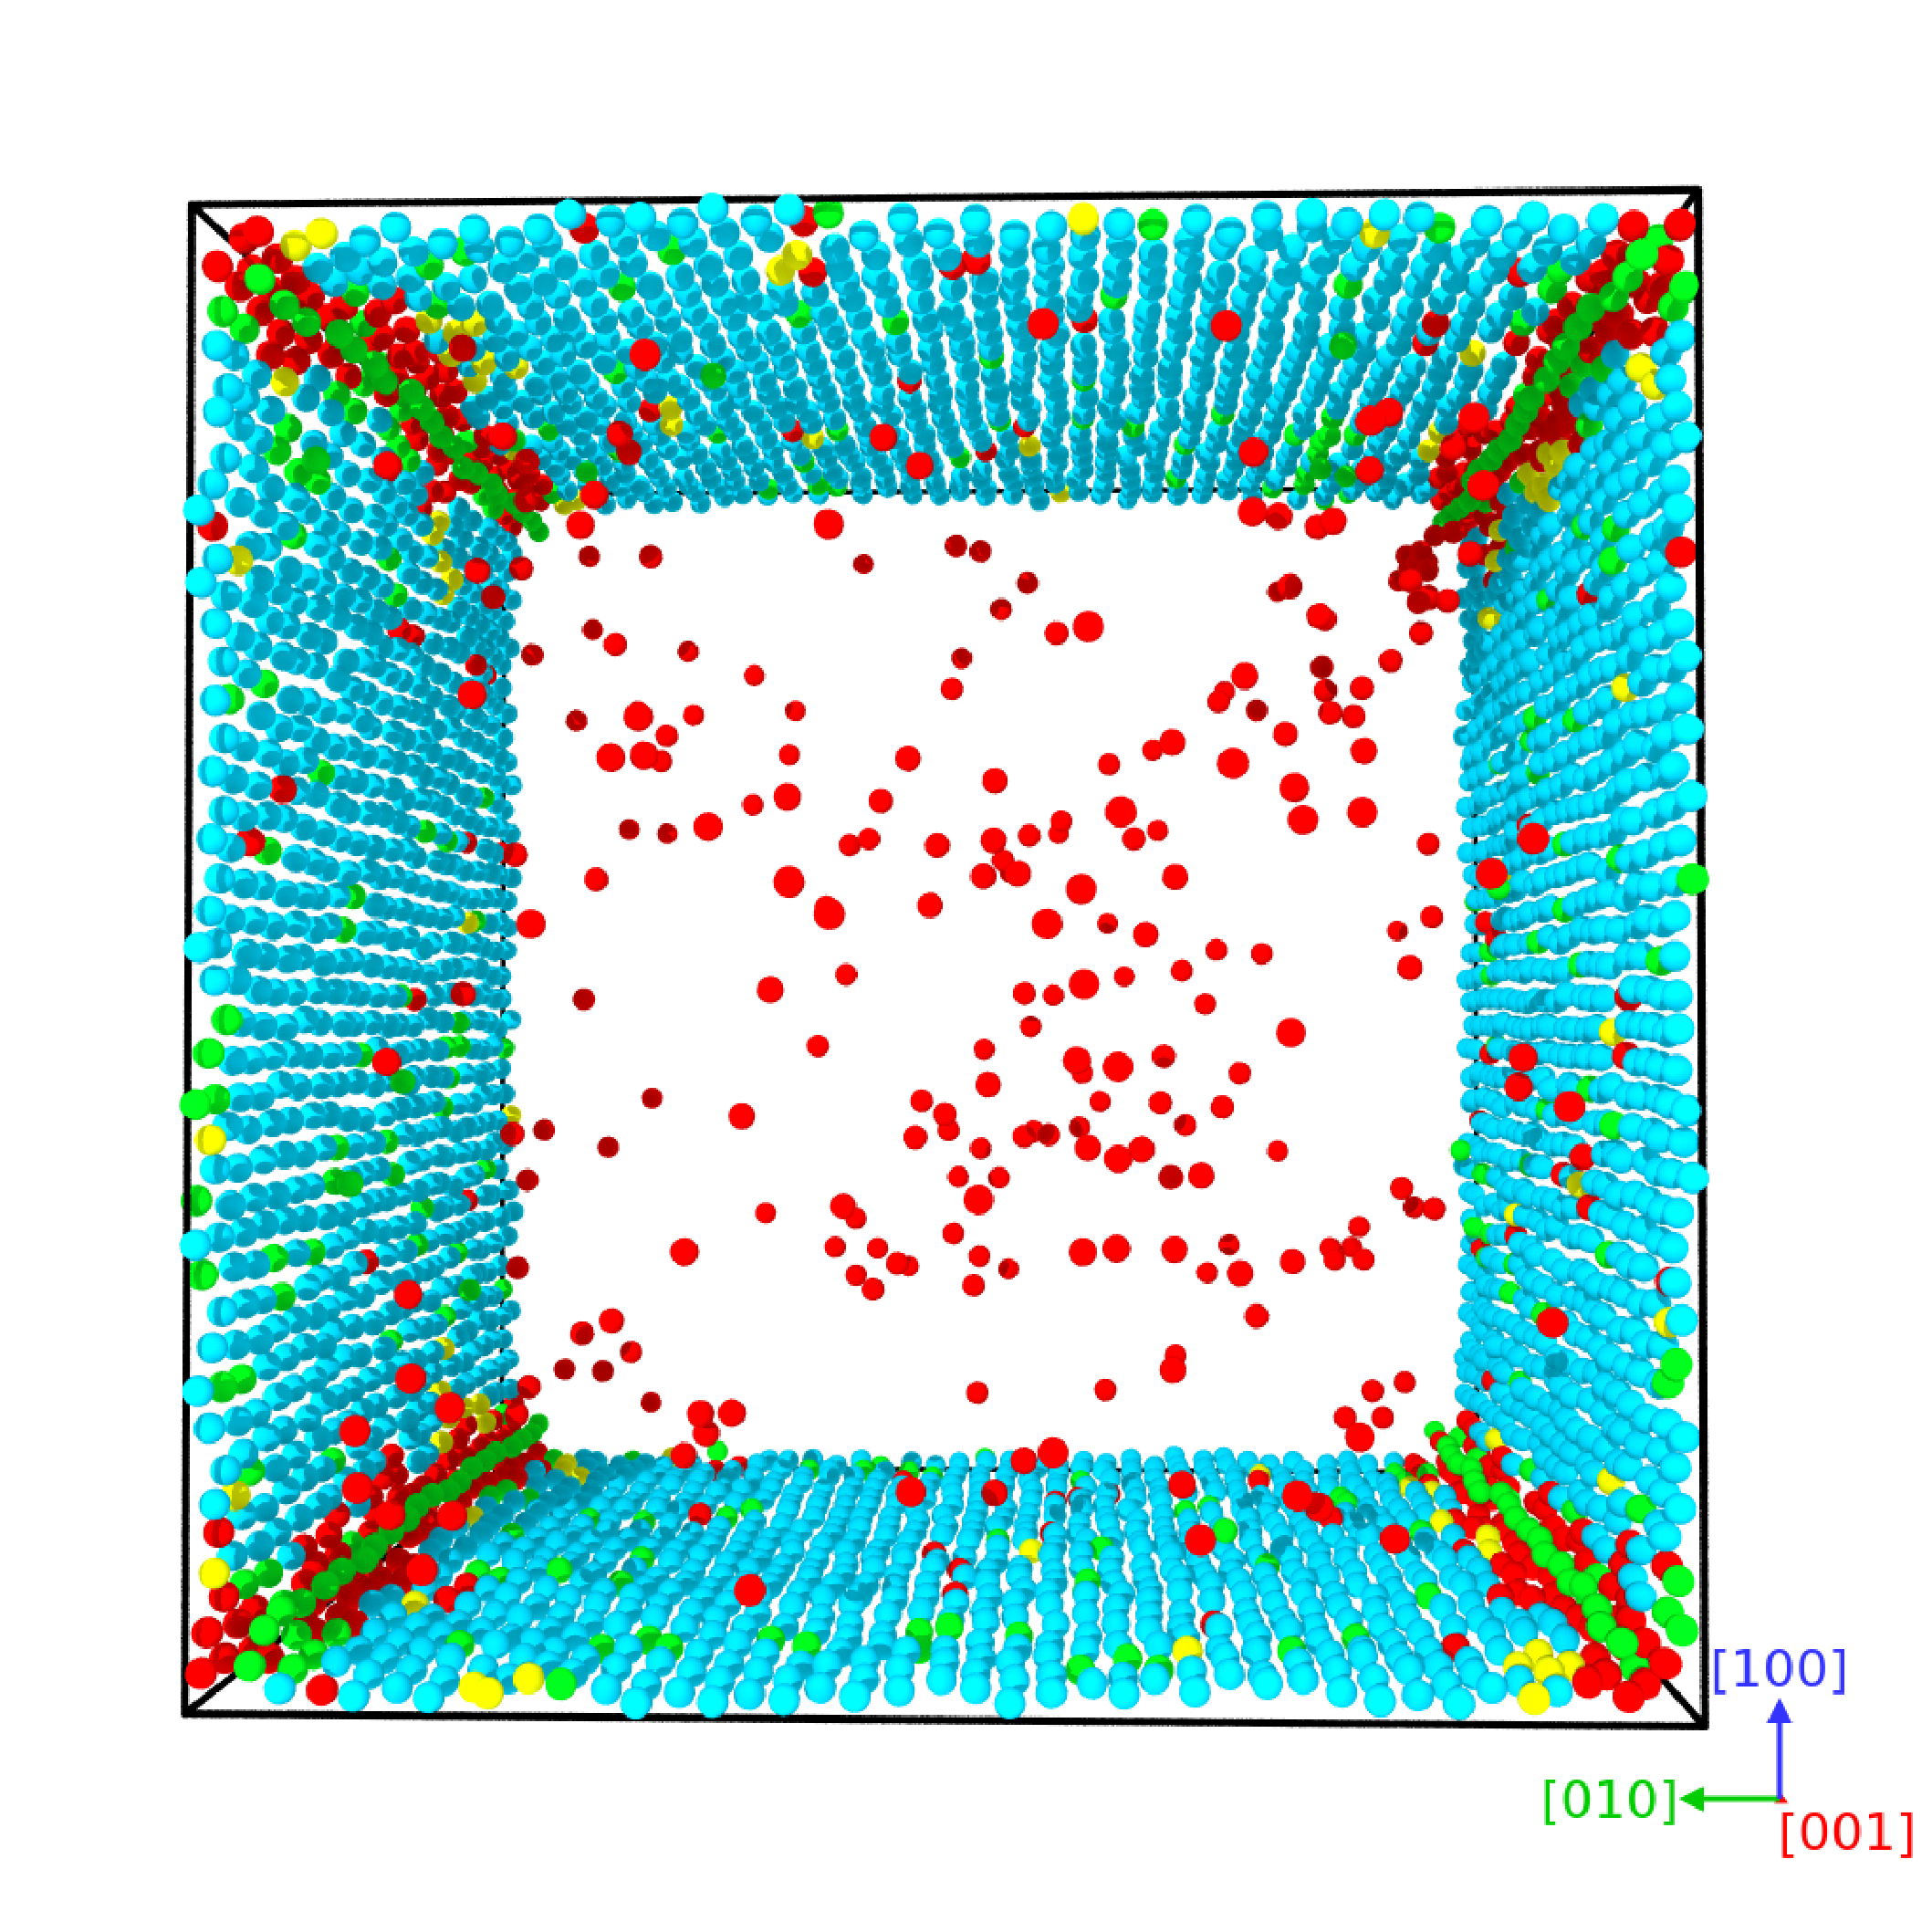
\includegraphics[width=7cm]{Figures/fcc_noise_bidef.png.eps}} \\
\subfloat[]{\label{fig:cnanoise}
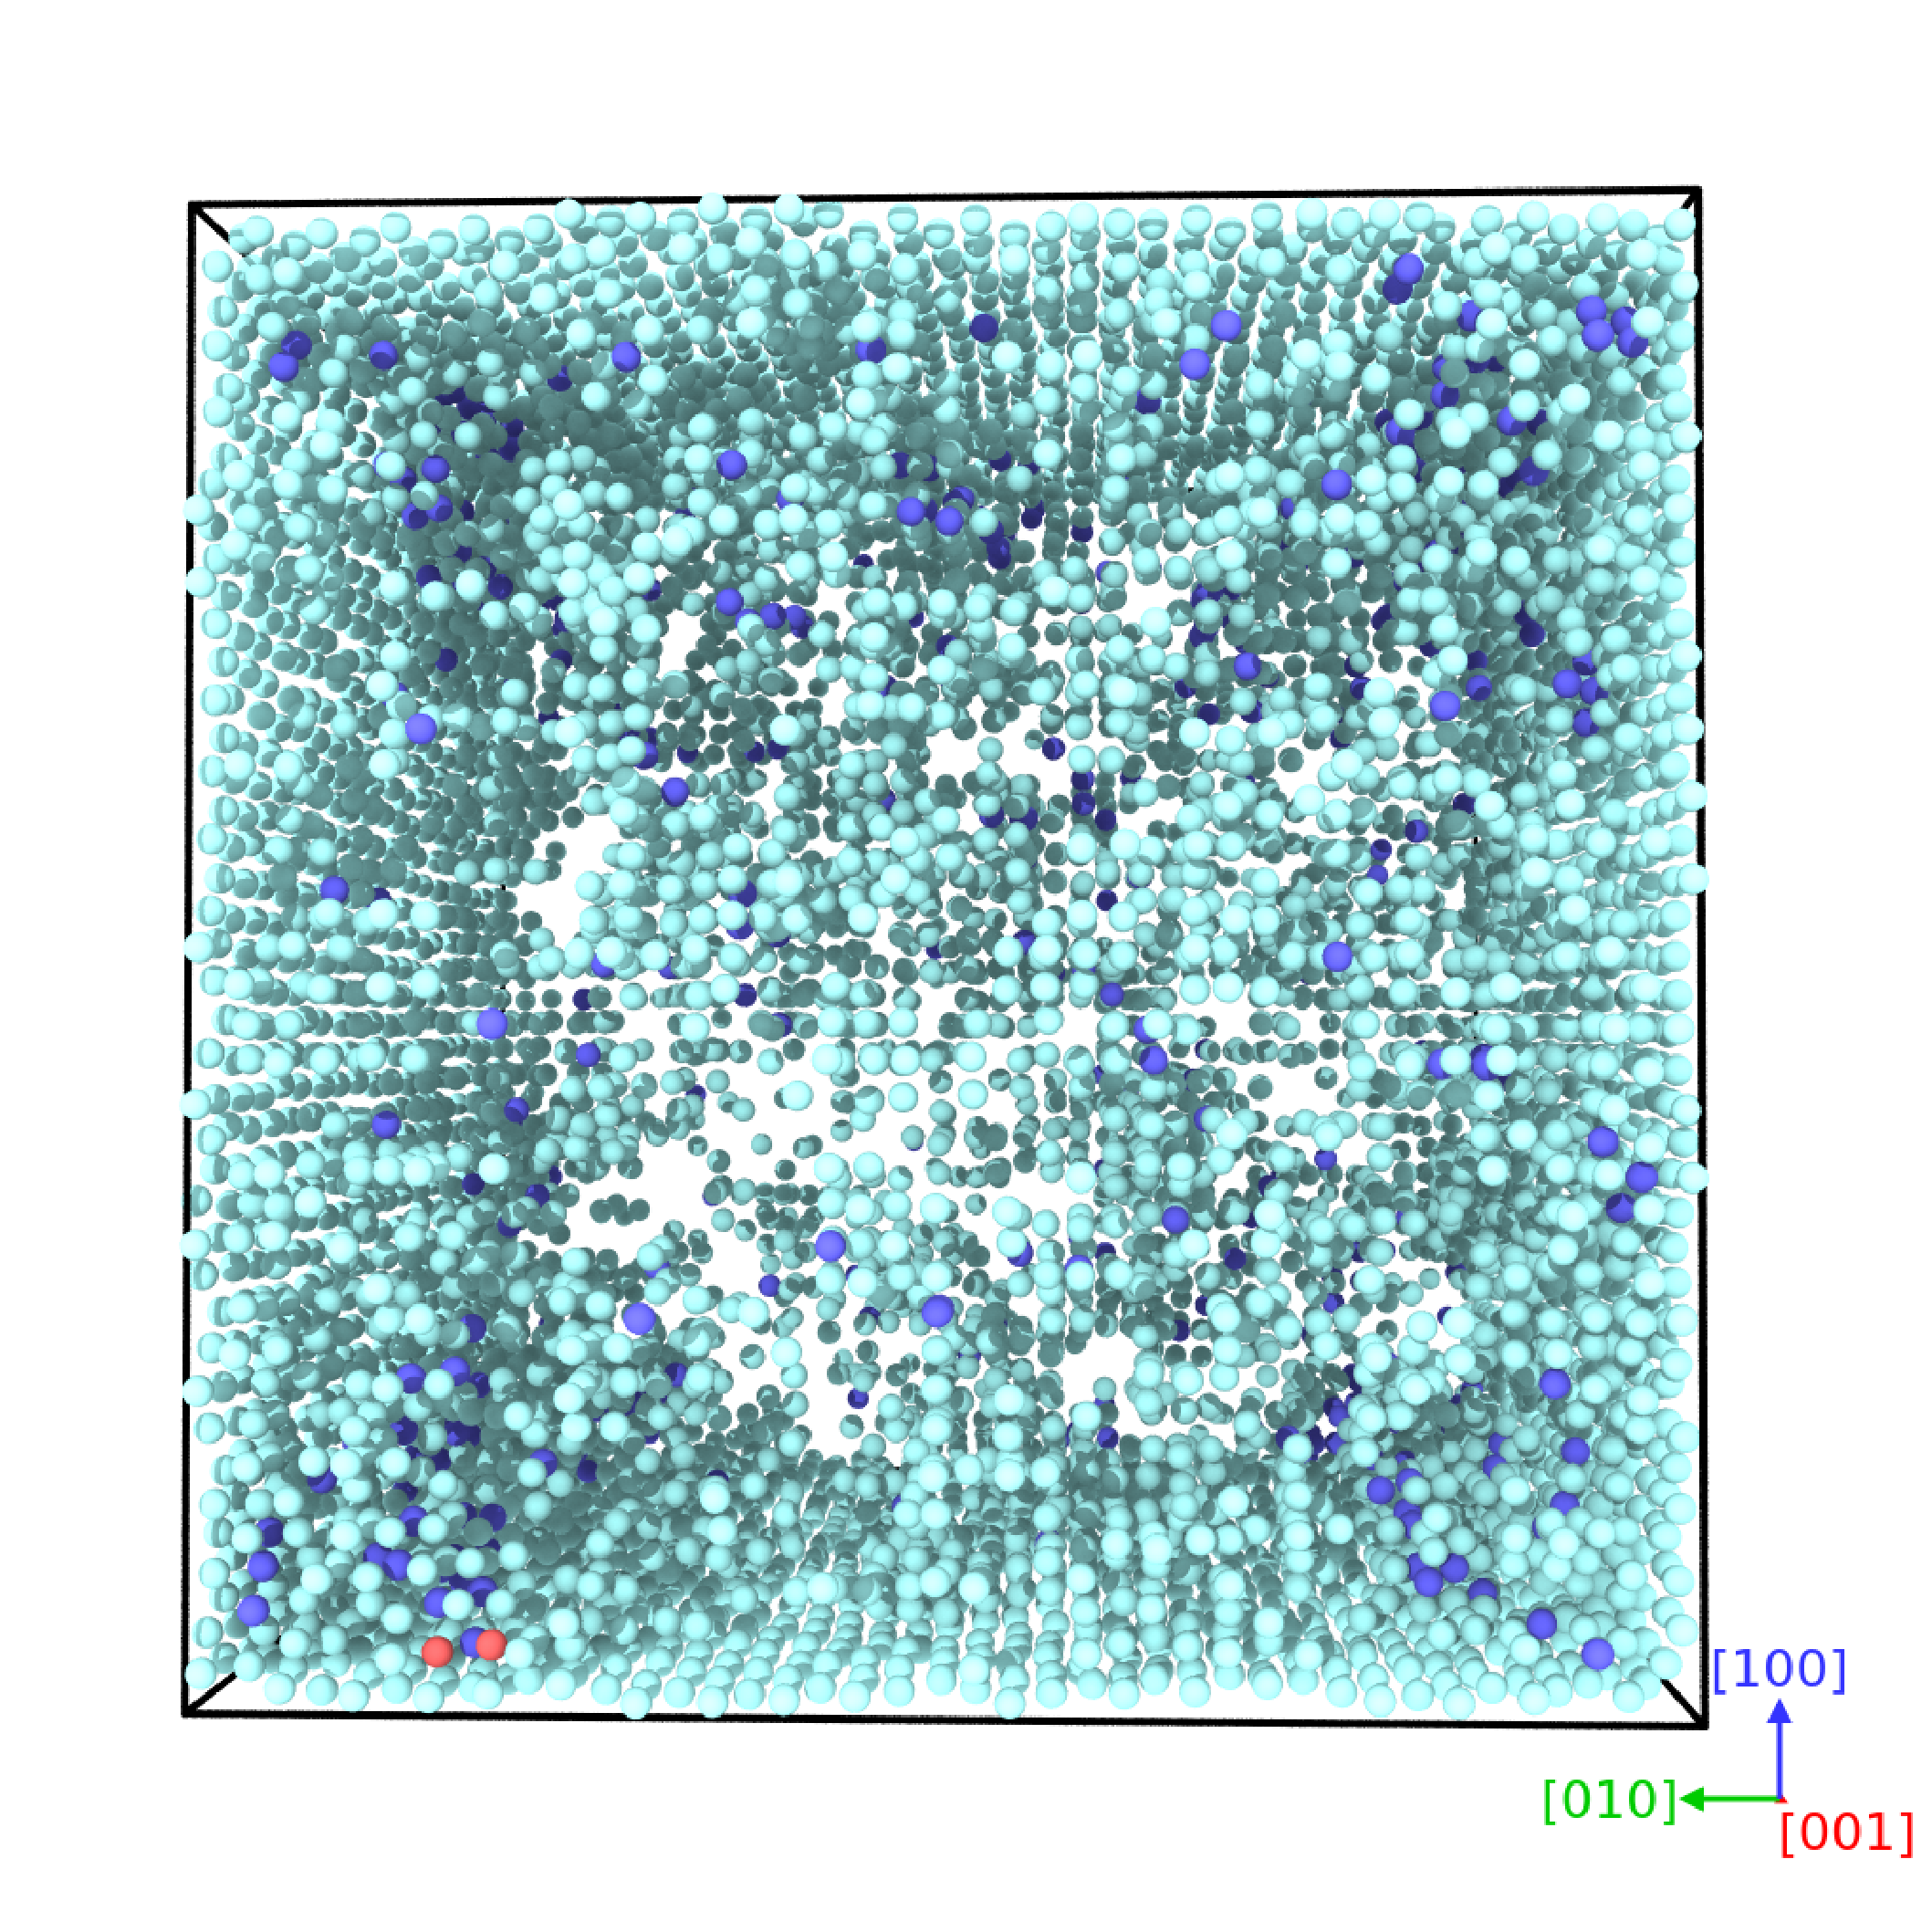
\includegraphics[width=7cm]{Figures/fcc_noise_cna.png.eps}}
\caption{Pre-yield tensile FCC cell noise comparision between a) BiDef and b) CNA. This sample was at 500K and compared before slip had occured. Atoms identified as bulk sites (FCC) are removed from the figure to observe noise in identification.}
\label{fig:bcc_noise}
\end{center}
\end{figure*}

Fig.\ref{fig:errorfcc} gives an error comparision between CNA and the BiDef algorithm for the FCC tensile test. Using our error identifcation method, the misidentification error is exclusively higher when using the CNA method as compared to the BiDef algorithm. After yielding the algorithms appear similar in Fig.\ref{fig:errorfcc}. However, when examing the defect structures, we found that CNA identified many regions as 'other' where no apparant slip had occured. A disdvantage of our error evaluation method is apparant when large neighboring areas of atoms are mis-idenfied. Since they are surrounded by defect atons, they won't be labeled as erroneous. Fig.\ref{fig:bispecnoise} shows a snapshot of the FCC cell, for both algorithms, at 500K. It is clear from this figure that regions which were identified as 'other' sites in the CNA method, are actually bulk locations at large strain (the yield stress had yet to occur). The BiDef algorithm appears to be superior at avoiding the misclassification of these sites.

Another verification study was performed using vacancy diffusion at relatively high temperatures in a square 72 $\AA x \AA  x \AA$ FCC copper nanowire simulation (1 periodic dimension). 106 vacancies were inserted randomly into the lattice, and a simulation was performed for 100 picoseconds at 900K to allow the vacancies to equilibrate. Qualitative differences in defect idenfication error can be observed in Fig.\ref{fig:vacancy_structures}. Since non-defective (FCC) atoms are removed in Fig.\ref{fig:vacancy_structures}, it is clear that significantly more defective sites are identified using the CSP (with a cutoff of CSP=5) and CNA methods than the BiDef algorithm. As with the previous simulations, the BiDef algorithm was capable of differentiating surface atoms, bulk atoms, and vacancy adjacent atoms within a margin of error.

\begin{figure*}
\begin{center}
\subfloat[]{\label{fig:bidefvac}
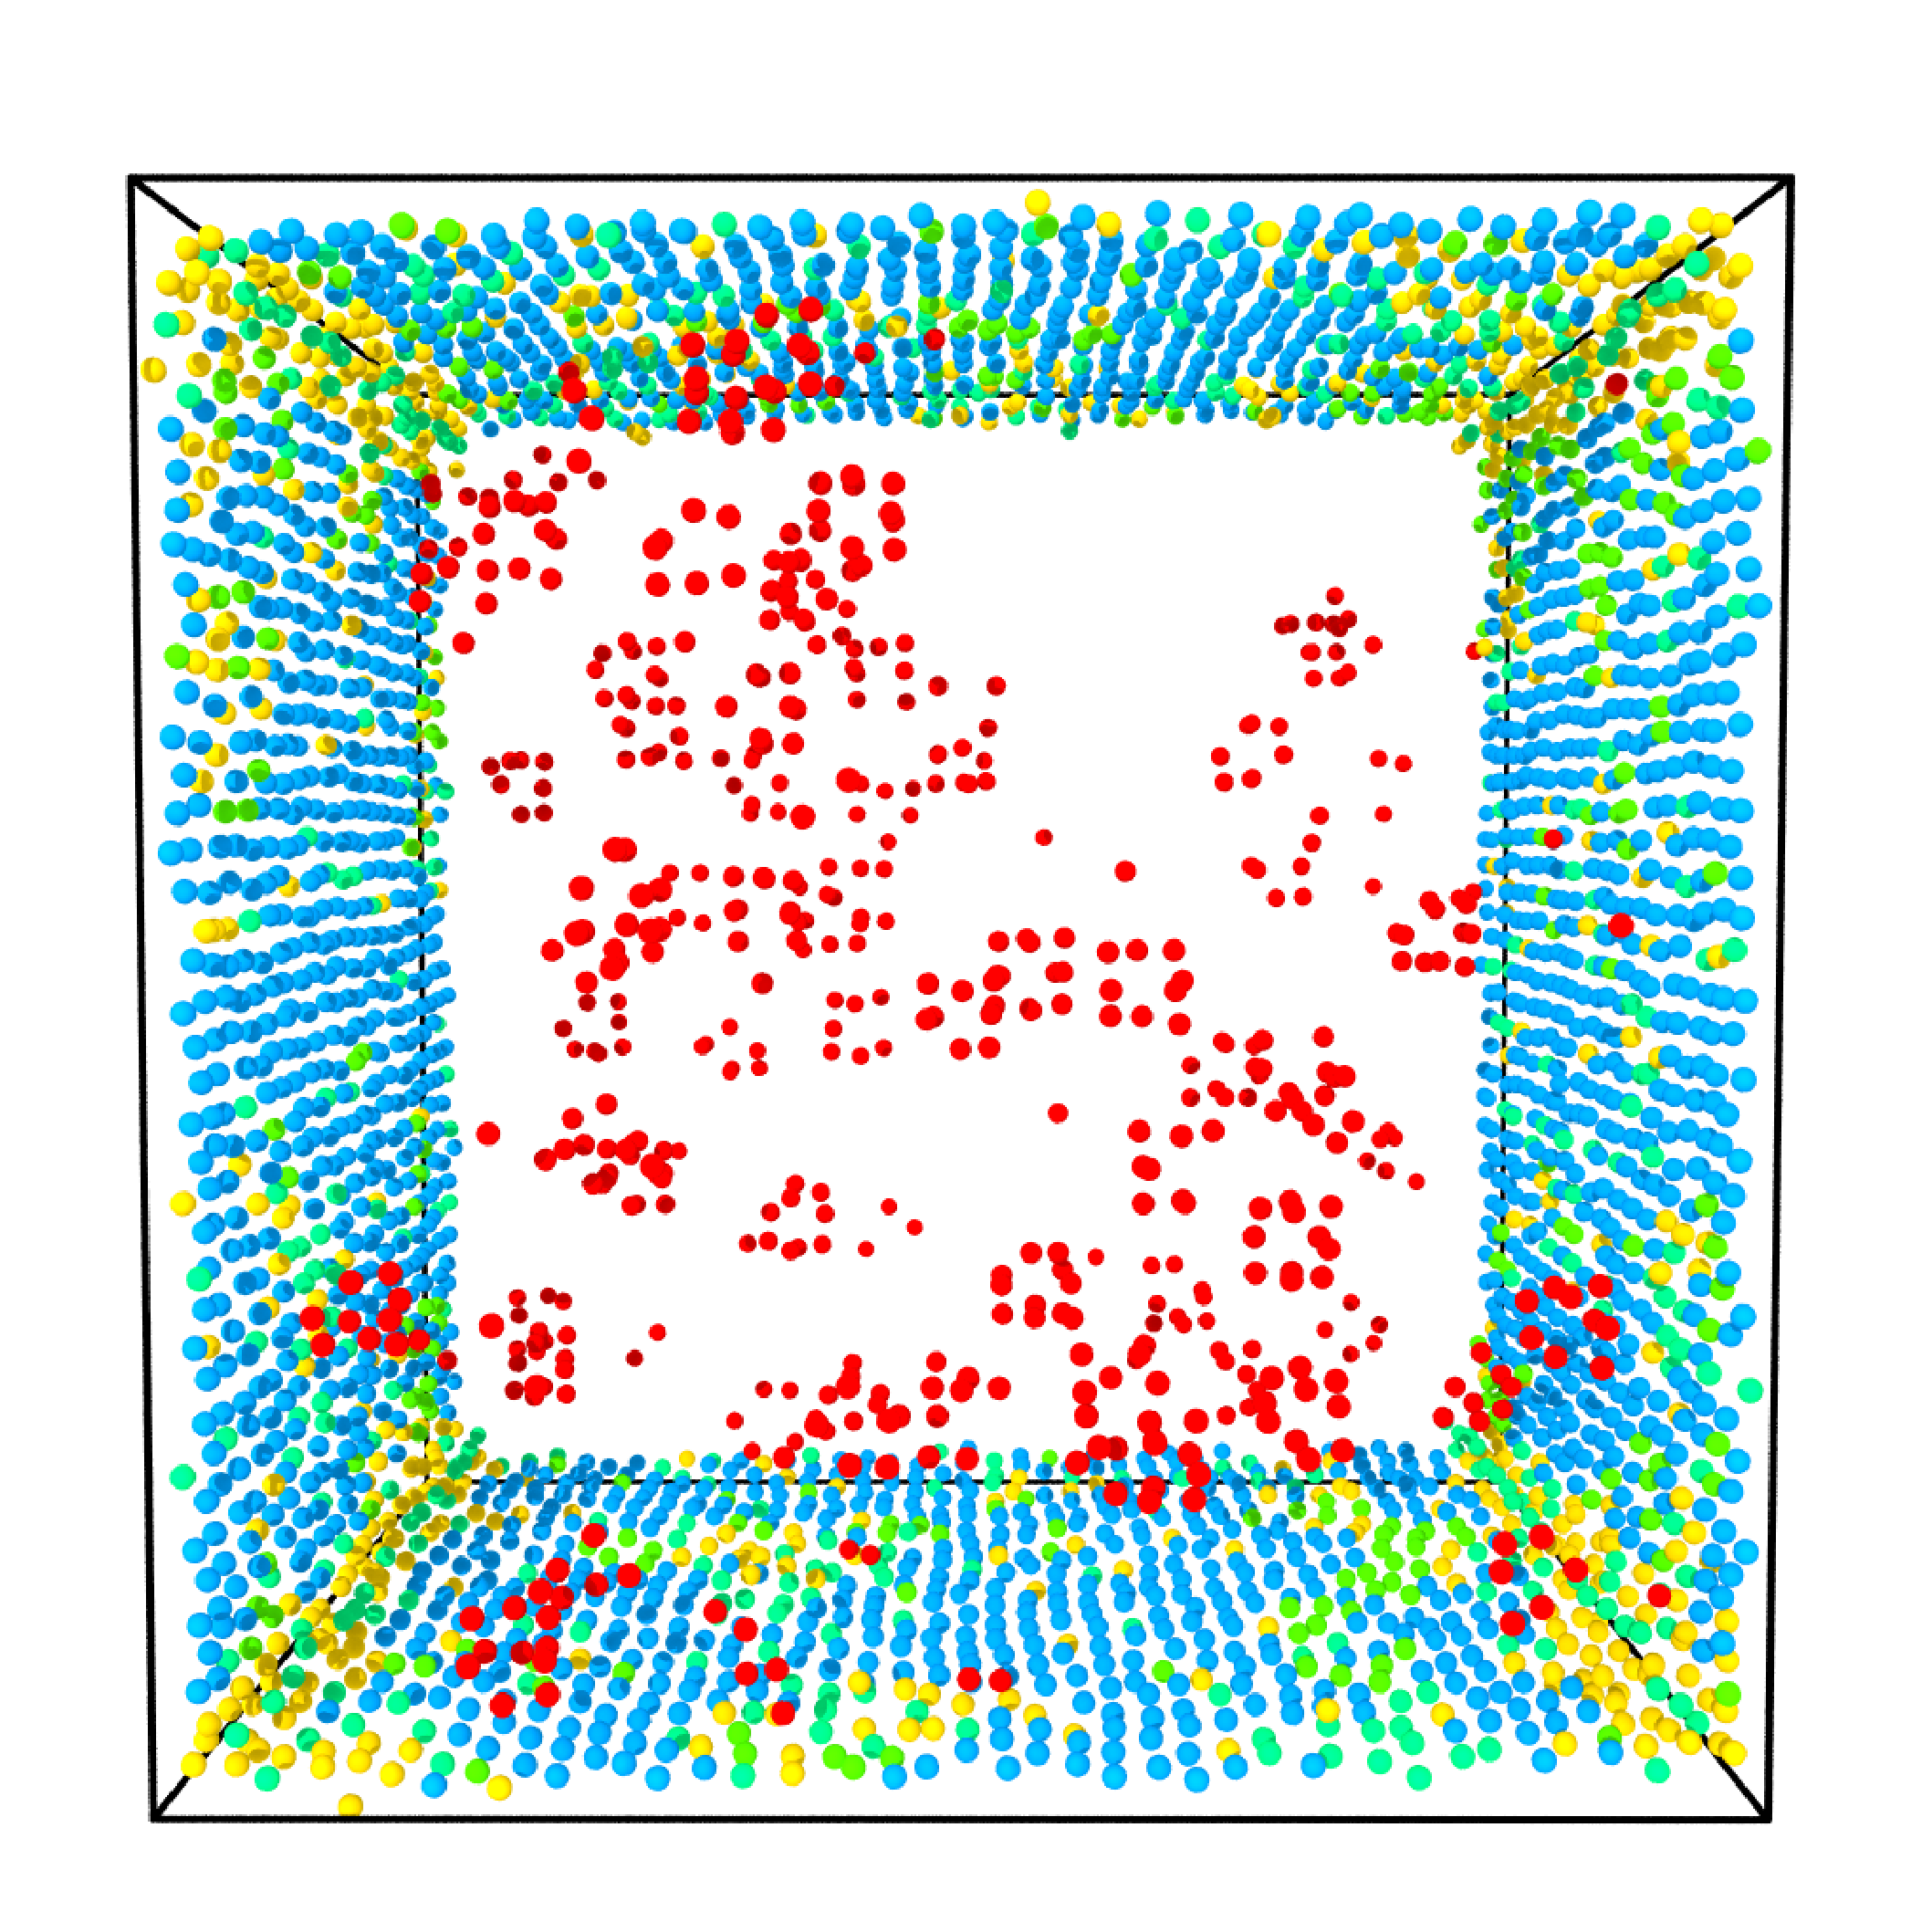
\includegraphics[width=7cm]{Figures/vacancies_render_bidef.png.eps}} \\
\subfloat[]{\label{fig:cspvac}
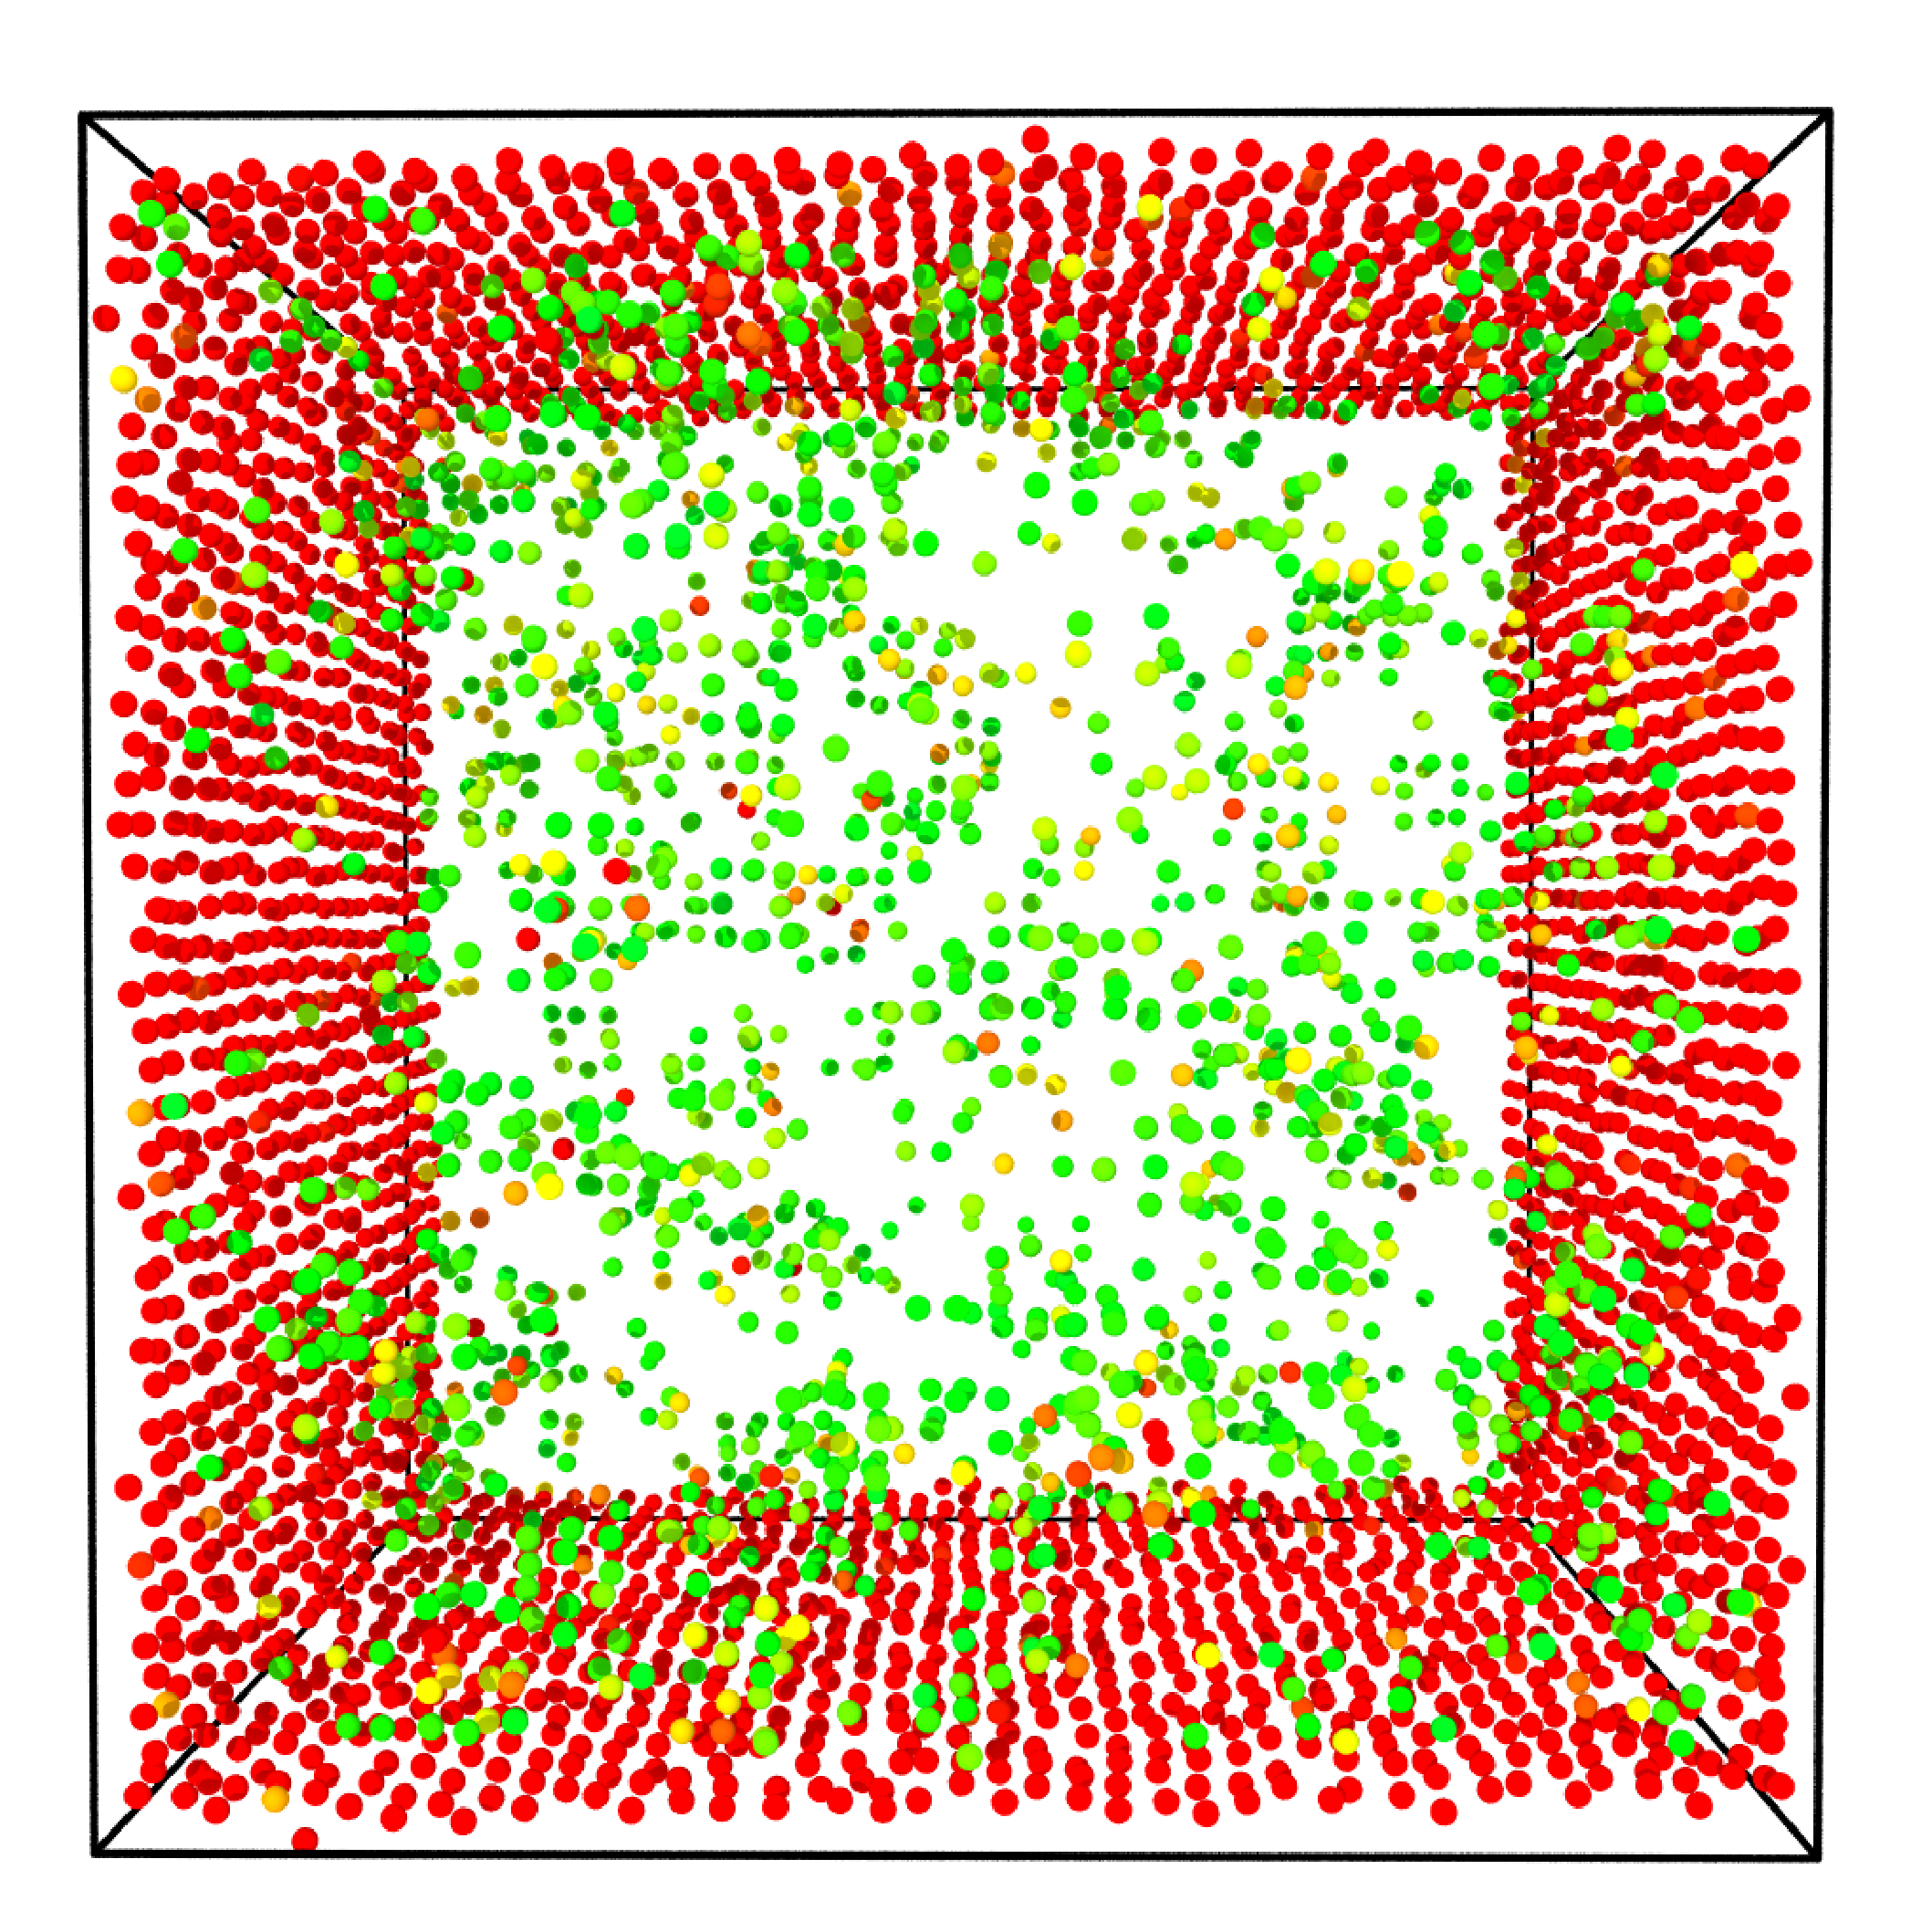
\includegraphics[width=7cm]{Figures/vacancies_render_csp.png.eps}}
\subfloat[]{\label{fig:cnavac}
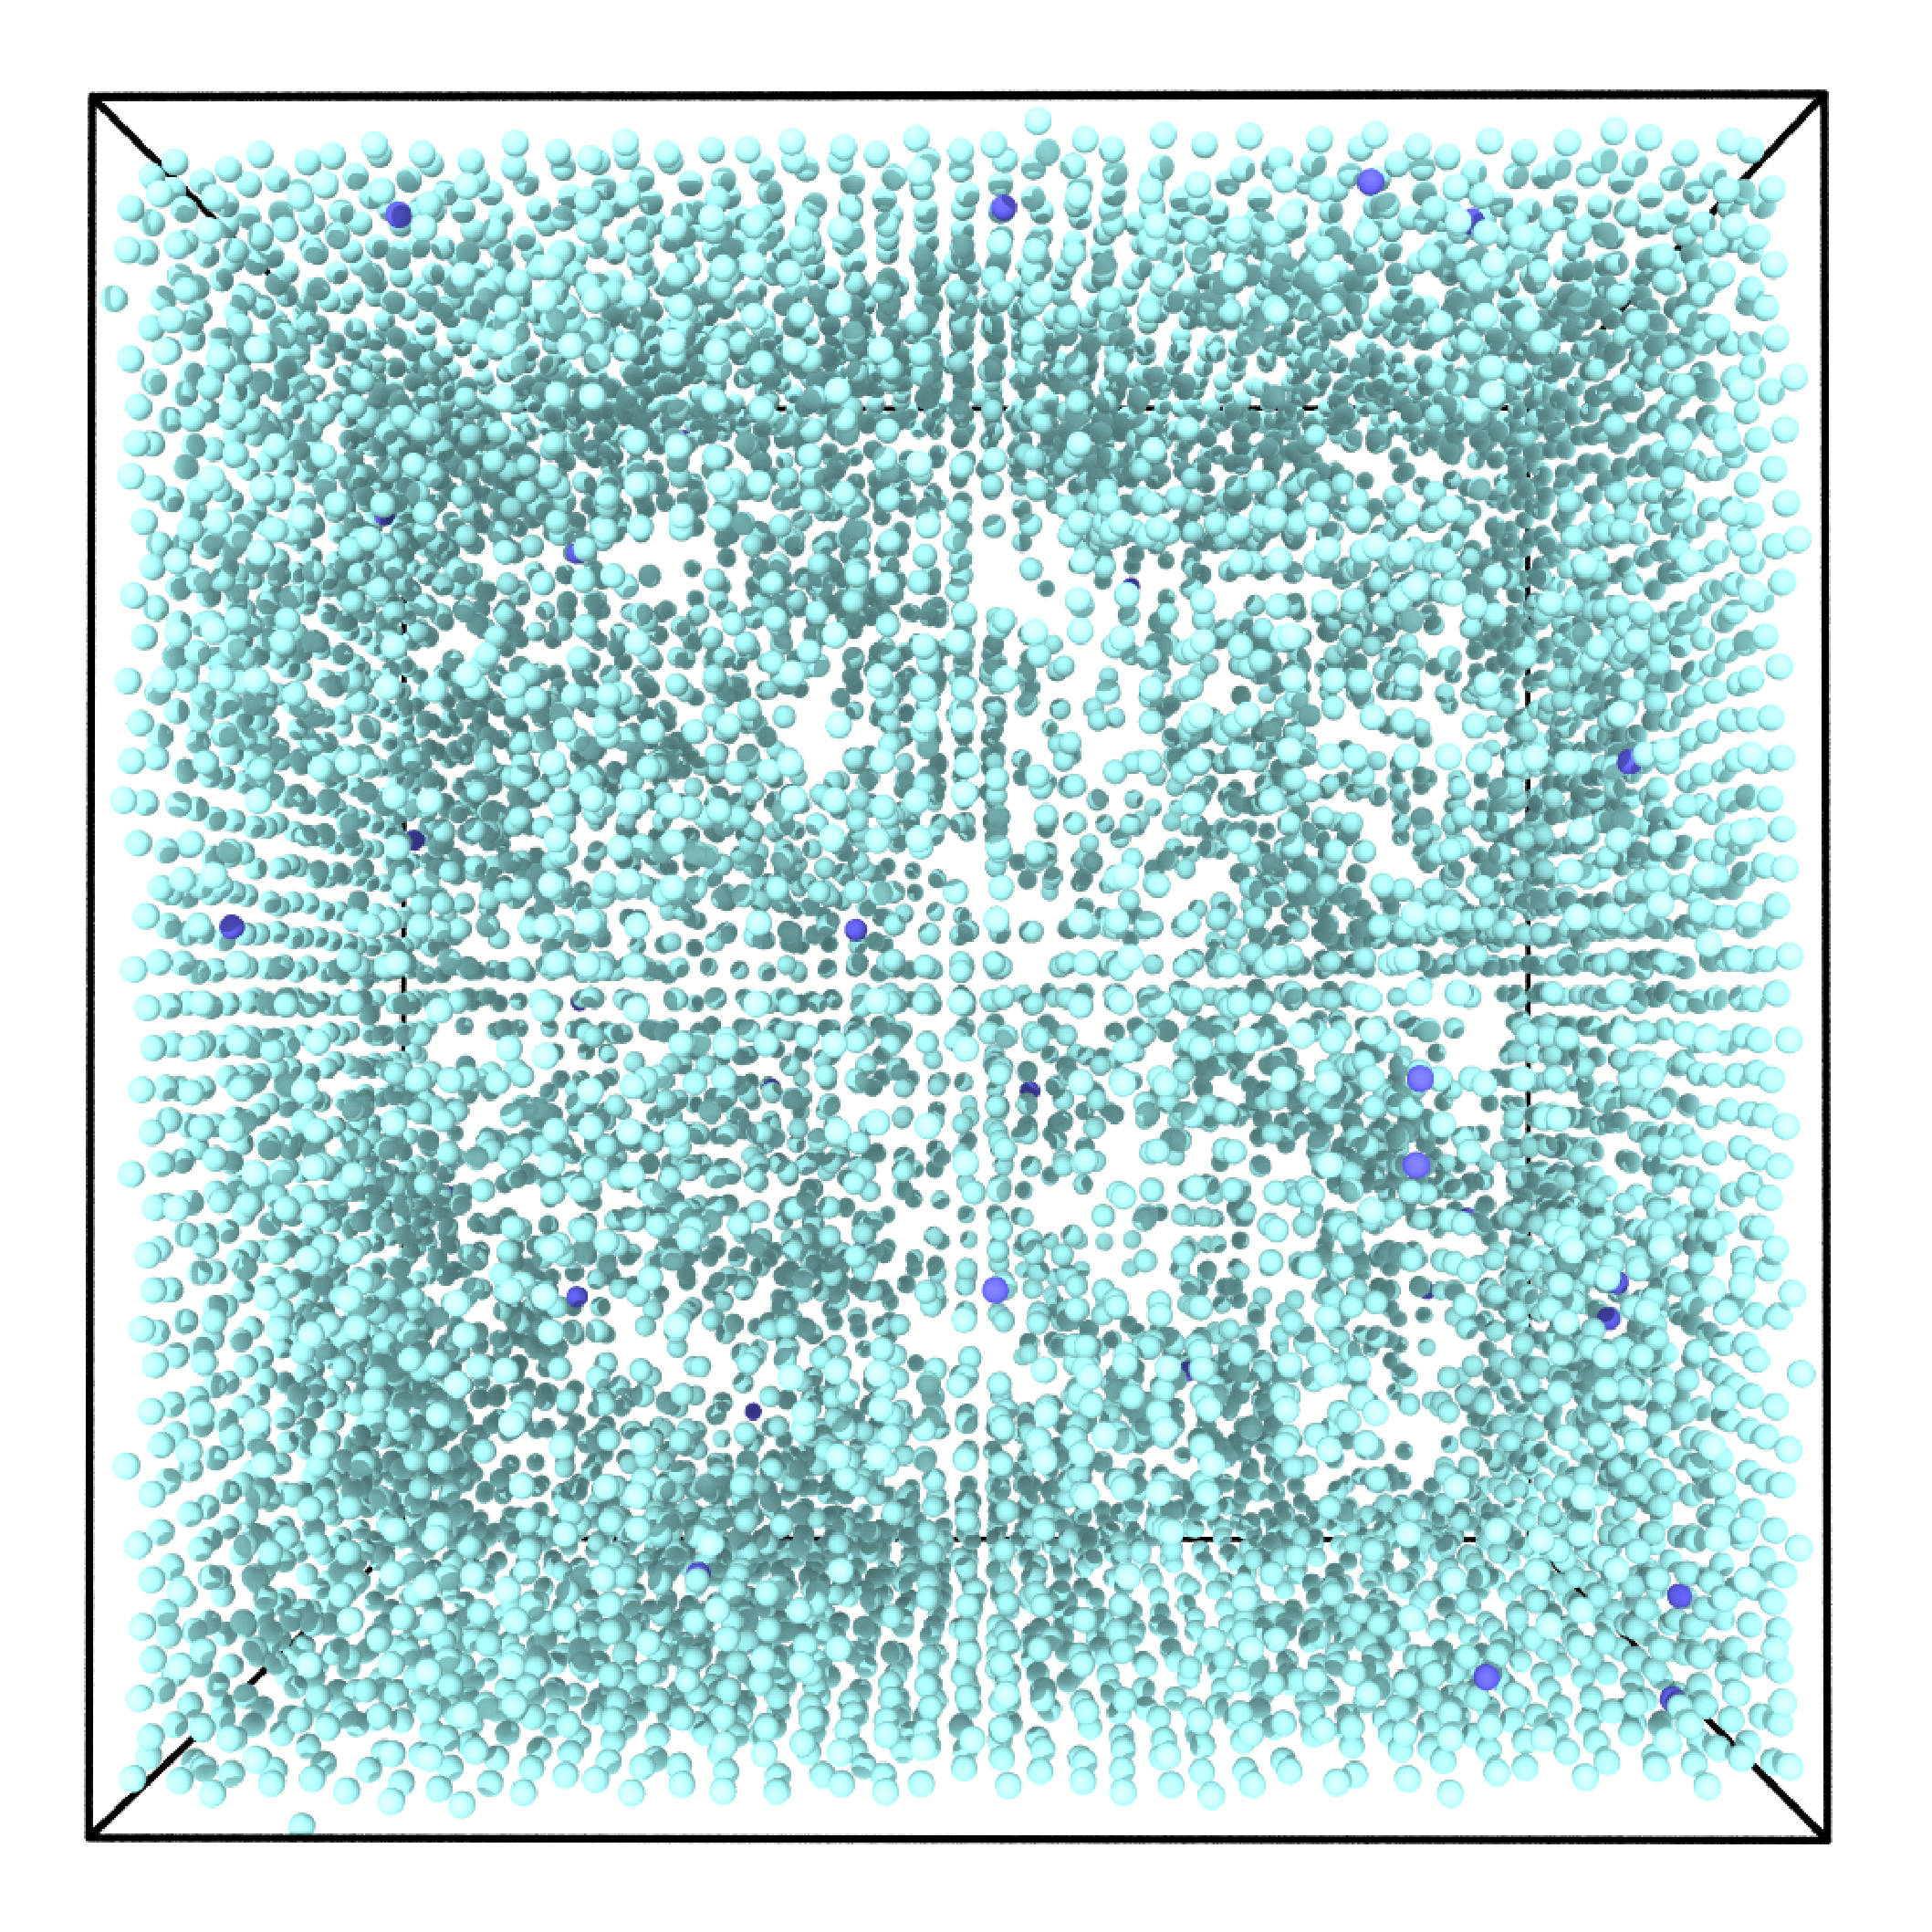
\includegraphics[width=7cm]{Figures/vacancies_render_cna.png.eps}}
\caption{Defect identification differences for vacancies inserted into copper FCC nanowire at 900 K. a) BiDef method, colored such that red atoms are an FCC vacancy, and yellow and blue atoms are (112) and (100) surfaces, respectively. All sites identified as FCC have been removed. b) CSP colored scheme where all atoms with a CSP value less than 5 have been removed. c) CNA colored scheme with all atoms identified as FCC removed, leaving the eggshell color as non-identified lattice structure.}
\label{fig:vacancy_structures}
\end{center}
\end{figure*}

An error calculation was necessary to quantitatively compare the algorithms. It is possible for these algorithms to falsely identify defective (false positive) and non-defective sites (false negative), so we used coordination data to evaluate the error for each algorithm. False positive sites were determined by first examining coordination, where a site labeled as defective would be incorrectly identified if the coordination number remained at 12, and then testing for the number of nearest neighbors which were also identified as defective. Defective sites without any defective nearest neighbors were likely mislabled as a vacancy would be surrounded by atoms with a lowered coordination. False negative sites were found by examining the number of 'bulk' sites that had lowered coordination ($<12$), while also having a defective nearest neighbor. Surface sites were eliminated from the error calculations for the CSP and CNA method by not counting atoms with coordination numbers less than 9 in these simulations. This actually improves the calculated error for the CNA and CSP algorithms as surface atoms typically have lower coordination numbers than the chosen cutoff. 

False negative and false positive defects were summed for each simulation technique and normalized to the number of sites in the simulation such that they could be directly compared with an error percentage, as shown in Fig.\ref{fig:errorvacancy}. While the system equilibrates ($<20$ ps), we see that the errors are very low, indicating that thermal fluctuations produce a majority of the erroneous classifcations in all three methods. Furthermore, while the temperature is increasing, both CNA and CSP methods produce less erroneous classifications than the BiDef method, up until about 7 ps. After this point, the thermal fluctuations produce much larger errors in the CNA and CSP methods. A pleateu is reached upon equilibration, near 30 ps, where the errors remain constant as the simulation progresses. At this point the BiDef method had an error of $2.58 \pm 0.16 \%$, the CNA method had an error of $9.91 \pm 0.23 \%$, and the CSP method had an error of $8.29 \pm 0.23 \%$. Even when considering both false negative and false positive defect identification, the BiDef method was considerably more accurate at finding atoms adjacent to vacant sites. This is compounded with the advantage that the BiDef method is able to determine these atoms as a separate classification from the surface and edge atoms, without further coordination analysis. This would allow for tracking of just the vacancy adjacent atoms during a simulation.

\begin{figure}[htbp]
  \centering
    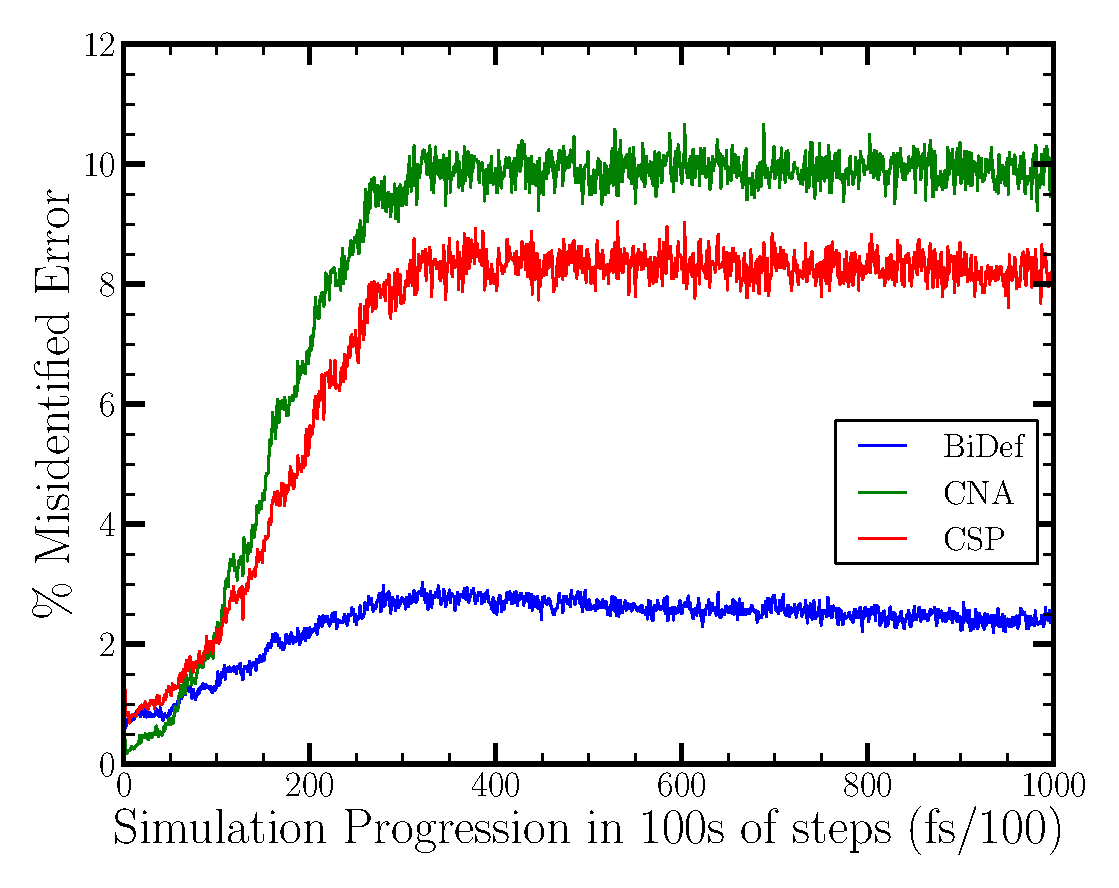
\includegraphics[scale=0.50]{Figures/vacancy_error.eps}
    \rule{35em}{0.5pt}
  \caption[]{Misidentification error comparison between CNA, CSP, and BiDef algorithms in a vacancy filled copper nanowire.}
  \label{fig:errorvacancy}
\end{figure}

Disadvantages include the run-time speed, and the fact that it is selective to nearest neighbor selection region. Mention that is is easily capable of having multiple atom types, which add's to the algorithm's strenght in comparision to geometry-only methods as it will differentiate structures with compositional changes as well. Accuracy seems to be linked to NN cutoff distance, such that at intermediate values between nearest neighbor layers, the fluctuating NN count serves to obscure the training data, giving a less accurate fit. The problem is quite interesting and it can be seen in the samples with 'oxide' layers. When the oxide layers are removed, the sample is able to find the underlying structure. The system struggles when two crystalline systems are presented with differing lattice constants, local lattice differences produce changes in bispectrum components. Since the algorithm currently does not have a means of reconciling lattices with two different equlibrium size scales, BiDef is unable to identify these more complex lattice structures, which have not been previously seen in the training data. One solution to this issue would be to provide training data with FCC-BCC interface structures, which would be later identified by BiDef.  (I'm thinking I should just add this to the library... it wouldn't be that difficult and I think it would allow for this sort of thing to work well)



\section{Conclusions and Outlook}

From the preliminary tests presented here, it appears that using machine learning for defect identification is a promisng method which avoids several issues presente in other methods. Specifically, it's capable of uniquly identifying defects, has relative intolerance to temperature and strain, and can be modified to examine any new type of defect. The power of this method does come with some disadvantages, it is quite slow in comparision to other methods. This is primarily due to the time it takes to generate bispectrum components. Although this process can be parallized to increase performance. We examined both random forest and nearest neighbors as learning algorithms, and found random forests had superior performance, while being slower to execute. In our case studies, we found that the BiDef method was less noisy than both CNA and CSP for identifying tensile defects during yielding. However, the algorithm slightly underperformed CNA in identifying all of the slipped regions after yeilding in BCC systems. Hopefully, the flexibility of this methods encourages others to contribute more complex defects to its training library such that it becomes more capable with time. 

\section{Bibliography}

\bibliography{Bibliography}

\end{document}

